%!TEX encoding = UTF-8 Unicode
%!TEX program = arara
% arara: pdflatex: {synctex: yes}
% arara: komkindex: {style: kotex}
% arara: pdflatex: {synctex: yes}
%%
%%% file `kotexdoc.tex`
%% Written by Kangsoo Kim <karnes at ktug kr>
%%
%%  2013/09/30
%%  2013/11/07
%%  2014/03/01, \ksnamedef
%%
%% part of ko.TeX v3.0
%% LPPL, maintained.
%
\documentclass[a4paper,%
	10.5pt,%
	amsmath,%
%	uset1font,%
	chapter,%
	twoside,%
	openany,%
	finemath,%
	oldfontcommands]%
{oblivoir}

\usepackage{fancyvrb}
\usepackage{eurosym}

\ifPDFTeX
  \SetHanjaFonts{uhcmj}{nanumgt}{nanumgt}
  \usepackage[pdftex]{graphicx}
  \SetGremphFonts{nanumgt}{nanumgt}
  \usepackage[normalem]{ulem}
  \usepackage{dhucs-trivcj}
%  \usepackage{dhucs-midkor}
  \input sample-finemath-setup.tex
  \usepackage[T1]{fontenc}
  \renewcommand{\rmdefault}{nanummj}
\else
  \ifLuaOrXeTeX
  \usepackage{xob-dotemph}
  \setkormainfont(* ExtraBold)(*){NanumMyeongjo}(){HCR Batang LVT}
  \def\다{\nobreak 다}
\fi\fi

\usepackage[x11names,dvipsnames,svgnames]{xcolor}

\ifXeTeX
  \usepackage[normalem]{ulem}
\fi

\usepackage[dbl4x6]{fapapersize}
\usepackage{boxedminipage}

\SetHangulspace{1.5}{1.1}

\usepackage{hologo}
\usepackage{kotex-logo}
\usepackage{ruby}
\def\rubysep{-1ex}
\def\pdfTeX{\hologo{pdfTeX}}
\def\pdfLaTeX{\hologo{pdfLaTeX}}
\def\XeTeX{\hologo{XeTeX}}
\def\XeLaTeX{\hologo{XeLaTeX}}
\def\eTeX{\hologo{eTeX}}
\def\LuaTeX{\hologo{LuaTeX}}
\def\LuaLaTeX{\hologo{LuaLaTeX}}
\newcommand*\kotex{\texorpdfstring{\textsf{k}\kern-0.0625em\textit{o}\kern-1.5pt\lower.15ex\hbox{.}\kern-1pt\protect\TeX}{ko.TeX}}
\def\ko{\textsf{k}\textit{o}}
\def\kotexplain{\kotex-\hologo{plain}}
\newcommand\kotexversion{v3.0}
%\newcommand\kotexdate{2013년 11월}
\newcommand\kotexdate{2021년 7월}

%\usepackage[
%    backend=biber,
%    style=authoryear,
%    sortlocale=UTF-8,
%    natbib=true,
%    url=true, 
%    doi=false,
%    eprint=false,
%]{biblatex}
%\addbibresource{kotexguide.bib}
%\addbibresource{texbook1.bib}
%\addbibresource{texbook3.bib}
%

\def\util#1{\texttt{#1}\index{Utilities!#1}\index{#1}}
\def\pkg#1{\textsf{#1}\index{Packages!#1}}
\def\option#1{\texttt{[#1]}\index{Options!#1}}
\def\wi#1{#1\index{#1}}
\def\thispkg{\kotex}
\def\file#1{\texttt{#1}\index{Files!#1}}

\def\OMEGA{$\mathrm{\Omega}$}

\copypagestyle{part}{empty}

\renewcommand\cftsectionaftersnumb{\hspace{1.2em}}
\renewcommand\cftsubsectionaftersnumb{\hspace{1em}}

\def\xample{예시}
\renewcommand{\cmd}[1]{\cmdprint{#1}%
  \index{Commands!\string\cmdprint{\string#1}}}

\makeindex

\usepackage{kotex-varioref}

\begin{document}

\frenchspacing

\title{\kotex-utf~\kotexversion~사용 설명서}
\author{김강수}
\date{\kotexdate}

\begin{titlingpage}
\maketitle
\end{titlingpage}

\frontmatter
\tableofcontents*


\mainmatter
\pagestyle{hangul}


%\part{\kotex-utf 사용설명}\label{part:two}

\part{\kotex-utf 사용설명서}\label{part:two}

\section*{3.0에서 달라진 점}
\addcontentsline{toc}{section}{3.0에서 달라진 점}

2021년 7월의 \kotex\ 3.0에서 다음과 같은 점이 달라졌다.
\begin{itemize}
\item 2020년 10월 이후의 \LaTeX\ 포맷의 변경에 따른 내부 코드의 수정
\item \pkg{siunitx} 패키지와의 충돌 해결
\item label에 한글 사용 가능
\item 장절 표제의 형식을 다른 \koTeX\ 패키지 군과 일치하게 수정하고
이전 형식을 사용하기 위한 \pkg{kotex-sections} 추가
\end{itemize}

\chapter{유니코드 문서 작성하기}

\section{개관}

\kotex-utf는 \wi{UTF-8} \wi{유니코드}로 입력되는 한글을 \LaTeX\ 문서에서
식자하고 조판하게 하려는 스타일 패키지로서, 그 핵심 부분인 \pkg{kotex-utf.tex}을
\wi{김도현}이 작성하였다.

\section{첫번째 문서}
\subsection{간단한 문서 작성}
그림~\ref{fig:firstdoc}\과 같은 간단한 문서를 작성해보자.
\begin{figure}[tbp]
\begin{Verbatim}[fontsize=\small,numbers=left]
\documentclass{article}

\usepackage[hangul,nonfrench,finemath]{kotex}
\usepackage{dhucs-nanumfont}

\usepackage[colorlinks]{hyperref}

\begin{document}

\section{들어가기}
처음 문서를 작성합니다.

\end{document}
\end{Verbatim}
\caption{첫번째 문서, 예제}\label{fig:firstdoc}
\end{figure}

제3행에서 \texttt{kotex} 패키지를 \cmd{\usepackage}한다.
\kotex 의 모든 패키지는 이 wapper를 통하여 호출된다.
\pdfLaTeX 이 실행되고, 옵션이 없으면 이 스타일은 \pkg{kotex-utf.sty}를 부른다.
%(\pageref{\}페이지 \ref{sec:kotexsty}절을 보라.)
%또한 대부분의 contrib 패키지의 명칭은
%\texttt{dhucs-}로 시작한다. 

제8행 이후에서 \pkg{hyperref}\을 로드한다. 
%반드시 \option{unicode} 옵션을 주어야 한다. 
\wi{bookmarks} 설정은 \pkg{hyperref}의 default이므로 별도로 지정하지 않아도
책갈피가 만들어진다. 만약 책갈피를 만들지 않고자 한다면
옵션에서 \verb|bookmarks=false|라고 한다.
\cmd{\hypersetup} 명령을
이용해서 설정값을 추가할 수도 있다.
%\footnote{%
%  hangul-ucs 4.0 이전 버전에서는 \texttt{dhucs-ucshyper}라는 
%  부가 패키지가 제공되었으나, hyperref의 기능 향상에
%  따라 불필요해졌으므로 \kotex 에서는 이 부가 패키지를 제공하지
%  않는다.}

%제7행 이후의 \verb|\ifpdf .. \else .. \fi| 구문은 pdf\LaTeX 의
%실행 여부에 따라 서로 다른 설정을 하는 부분이다. 이 구문을
%사용하려면 \pkg{ifpdf}\가 필요하다. 
%주로 컴파일 루트가 \util{pdflatex}으로부터 직접 \file{pdf}를 얻는 
%것이 아니라 \util{dvipdfmx}를 이용하여 \file{dvi}를 \file{pdf} 변환하는
%방식으로 작업할 때를 위하여 이런 구문을 쓴다.

%제9행은 pdf\LaTeX 에서 텍스트의 검색\cntrdot 추출을 가능하게
%하는 행이다. 
%DVIPDFM$x$를 위해서는 별도의 설정이 필요없다.

%제4행부터 제8행까지는 반드시 필요한 경우가 아니면 꼭 지정하지 않아도 상관없다.
%각 (부가) 패키지의 작용 등은 이 문서를 읽으면 알 수 있다.
%제5행은 \pkg{dhucs-interword}\를 로드했기 때문에 선언한
%것으로서 이에 관련된 문제는 \pageref{sec:interword} 페이지의
%\ref{sec:interword}절에 설명되어 있다. 

이 내용을 \file{firsttest.tex}이라는 이름으로 저장한다.

\subsection{컴파일}

이 문서를 \wi{컴파일}하려면 \wi{명령행}에서 다음과 같이 한다.
\begin{Verbatim}[fontsize=\small]
$ pdflatex firsttest
\end{Verbatim}

또는 (선택한 작업 루트에 따라서) \util{latex}으로 얻어진 \file{.dvi}에 대하여 \util{dvipdfmx}를
실행한다.
\begin{Verbatim}[fontsize=\small]
$ latex firsttest
$ dvipdfmx firsttest
\end{Verbatim}

\subsection{옵션들}
\kotex-utf가 제공하는 옵션은 다음과 같다.
\begin{description}
\item[\texttt{hangul}]
한글 문서 서식을 설정한다. \wi{장과 절 포맷}은 ``제 1 장''과 같은 형태로 
식자된다. 기본값은 한글 문서 서식을 설정하지 않는 것이다.
\item[\texttt{nojosa}]
자동조사 기능을 끈다. dhucs 초기 버전에서 다른 패키지와의 호환을
위하여 제공되었던 것이지만 현재는 굳이 이 옵션을 사용해야 할 필요가
거의 없다. 그러나 옵션으로서는 유지되고 있다.
\item[\texttt{hanja}]
한글 문서 서식을 설정하는 것은 \texttt{hangul} 옵션과 같으나,
한글 이름 대신 한자 이름을 사용한다.
\item[\texttt{nonfrench}]
한글 문장에 대해서도 non-french-spacing을 적용한다. 즉, 마침표 등의
뒤의 공백이 다른 공백보다 조금 더 길다. 기본값은 \wi{french-spacing}으로
식자하는 것이다.
\item[\texttt{finemath}]
원래는 문장 중의 수학 식과 이어지는
한글 사이에 적절한(fine) 간격을 부여하기 위한 것이었으나, 곧 
문장부호 등을 포함한 개념으로 확대되었다.
\item[\texttt{strictcharcheck}]
한글 폰트 가운데 \file{.tfm}은 있으나 해당 문자가 결락되어 있는
것이 있다. 이럴 경우에 에러를 보여주도록 하는 옵션이다. 이 옵션을
지시하지 않으면 문자가 없어서 식자하지 못한 것을 \file{.log}에 기록만
하고 에러는 발생시키지 않는다.
\end{description}

\section{몇 가지 한글화}

\subsection{기호문자 처리}
기호문자 중 일부에 대해서는 미리 식자방법을 정의해두었다.
½, ¼, ‥ 등의 문자와 같은 몇 가지 한글 기호문자는 \texttt{[hangul]} 옵션을
준 경우에 식자할 수 있다.

참고로 한글 기호문자에 \euro 가 있지만 이것은 
\pkg{eurofont} 또는 \pkg{eurosym} 패키지를 사용하여
\cmd{\euro}와 같이 입력하는 편이 좋다.

\begin{table}
\centering
\begin{tabular}{cccccccccc}
\hline
자판 & 1 & 2 & 3 & 4 & 5 & 6 & 7 & 8 & 9 \\ \hline
ㄱ   &  & !& '&,&.&/&:&;&?\\
     &  ^&_&`&|& ̄&、&。&·&‥ \\
     &  …&¨&〃&­&―&∥&\&∼&´ \\
     & ~&ˇ&˘&˝&˚&˙&¸& ˛ & ¡ \\
     & ¿ &  Ð \\ \hline
ㄴ & "&(&)&[&]&{&}&‘ & ’\\
   &“&”&〔&〕&〈&〉&《&》&「 \\
   &」&『&』&【&】 \\ \hline
ㄷ &+&-&<&=&>&±&×&÷&≠ \\
   &≤&≥&∞&∴&♂&♀&∠&⊥& ⌒\\
   &∂&∇&≡&≒&≪&≫&√&∽&∝\\
   &∵&∫&∬&∈&∋&⊆&⊇&⊂&⊃\\
   &∪&∩&∧&∨&¬&⇒&⇔&∀&∃\\
   &∮&∑&∏\\ \hline
ㄹ & $ & % & ₩ & F & ′ & ″ & ℃ & Å & ¢ \\
   & £ & ¥ & ¤ & ℉ &  ‰ & \euro & ㎕ & ㎖ & ㎗ \\
   &ℓ&㎘&㏄&㎣&㎤&㎥&㎦&㎙&㎚\\
   &㎛&㎜&㎝&㎞&㎟&㎠&㎡&㎢&㏊\\
   &㎍&㎎&㎏&㏏&㎈&㎉&㏈&㎧&㎨\\
   &㎰&㎱&㎲&㎳&㎴&㎵&㎶&㎷&㎸\\
   &㎹&㎀&㎁&㎂&㎃&㎄&㎺&㎻&㎼\\
   &㎽&㎾&㎿&㎐&㎑&㎒&㎓&㎔&Ω\\
   &㏀&㏁&㎊&㎋&㎌&㏖&㏅&㎭&㎮\\
   &㎯&㏛&㎩&㎪&㎫&㎬&㏝&㏐&㏓\\
   &㏃&㏉&㏜&㏆ \\ \hline
ㅁ &#&&&*&@&§&※&☆&★&○\\
   &●&◎&◇&◆&□&■&△&▲&▽\\
   &▼&→&←&↑&↓&↔&〓&◁&◀\\
   &▷&▶&♤&♠&♡&♥&♧&♣&⊙\\
   &◈&▣&◐&◑&▒&▤&▥&▨&▧\\
   &▦&▩&♨&☏&☎&☜&☞&¶&†\\
   &‡&↕&↗&↙&↖&↘&♭&♩&♪\\
   &♬&㉿&㈜&№&㏇&™&㏂&㏘&℡\\
   &®&ª&º \\ \hline
\end{tabular}
\caption{Windows 특수문자 입력방식에 의한 특수문자}\label{tab:symbols}
\end{table}

\wi{윈도우즈} 기본 \wi{한글 입력기}에서 \wi{특수문자}를 입력하는 방법은 `ㄱ', `ㄴ' 등의 키를
누른 다음 \texttt{[한자]} 키를 눌러서 선택하는 것이다. 이 방법으로 입력되는
특수문자의 예를 표~\ref{tab:symbols}에서 보였다.\footnote{%
	\texttt{\textbackslash DeclareUnicodeCharacter} 명령을 이용하여
	ucs의 문자 설정을 변경하는 방법도 있다.}
`ㅎ' 행에는 그리스 문자가 할당되어 있다. 텍스트 그리스 문자는
현재 본문 기본 한자 글꼴에 있는 것으로 식자되는데, 만약 더 나은
텍스트 그리스 문자가 필요하다면 \pkg{babel}\을 이용하여 입력하도록 한다.	
아무 옵션 없이 해보면 이러하다: Τεχνη.
%ή.

기호 문자의 직접 입력과 처리가 가능하기는 하지만, 적어도 legacy \TeX 으로 작업한다면
이 기호 문자를 문서에서 바로 입력하여 사용하는 것을 권장하지 않는다.
기호 문자를 써야 할 경우에는 알맞은 \LaTeX 의 기호 문자 명령으로
얻도록 하는 편이 낫다.\footnote{%
	단, 유니코드 텍 엔진(\XeTeX, \LuaTeX)을 사용하는 경우에는
	유니코드 문자 자체를 입력하는 쪽이 바람직한 경우도 있다.}

\subsection{우리말 이름}
\label{sec:names}\index{우리말 이름}

한글 문서는 외국어 문서와는 달리 몇 가지 보조적 \wi{서식}을
가지고 있다. \wi{장절 명령}이 별도로 짜여져야 하고, \wi{행간}이나
\wi{단어 간격}도 적절하게 배치되어야 한다.
이를 위하여 이 패키지는 \option{hangul} 패키지 옵션을 제공한다.
이 옵션이 지시되면 한글 이름, 한글 장절표제 등을 활성화하고
행간을 한글에 알맞게 설정한다. 
%또한, \wi{장절 명령}과 관련해서 %\kotex/euc와 동일한 
%\cmd{\kscntformat} 명령이 작동한다.
% <!-- 2014/03/01, ksnamedef -->
%\wi{한글 이름}과 관련해서 \cmd{\ksnamedef} 명령도 작동한다.
%이 명령의 의미와 사용법에 대해서는 \pageref{sec:names} 페이지의
%\ref{sec:names}절을 보라.

%\pageref{tab:names} 페이지 표 \ref{tab:names}\를 참고하라. 

%한글 문서에서 사용되는 각종 이름들을 일률적으로
%\cmd{\ksnamedef} 매크로에 의해 변경될 수 있도록
%하였다.
이러한 ``한글 이름''을 사용하려면 \option{hangul} 옵션을
지정하여야 한다.

예를 들어, 라텍에서
사용되는 `\refname{}'의 이름 `Reference'는 \cmd{\refname}에 지정되어
있다.  이를 우리말화 하는 방법은 다음과 같다.
\begin{verbatim}
   \renewcommand{\refname}{참고~문헌}
\end{verbatim}

%\texttt{[hangul]} 옵션을 준 경우 이 명령을 사용할 수 있다.

표~\ref{tab:names}에는 한글 라텍에서 한글화한 ``라텍 이름의 한글 및
한자화''가 나열되어 있다.  이 한글화는 \wi{전처리부}(preamble)에서 
위에 예를 든 것처럼
%\cmd{\ksnamedef}로 
재정의하면 원하는대로 변경된다.

\begin{table}[htbp]
  \leavevmode
  \centering
  \begin{tabular}{l|l|l}\hline
               \multicolumn{1}{c|}{라텍명령}   & \multicolumn{1}{c|}{한글 라텍(한글)}  & \multicolumn{1}{c}{한글 라텍(漢字)}  \\\hline\hline
           \texttt{today} & 1994년 3월 6일  & 1994年 3月 6日  \\\hline
        \texttt{enclname} & 동봉물          & 同封物          \\\hline
          \texttt{ccname} & 사본            & 寫本            \\\hline
      \texttt{headtoname} & 받는이          & 受信人          \\\hline
         \texttt{seename} & \verb+\+을 참고 & \verb+\+을 參考 \\\hline
    \texttt{contentsname} & 차\~{}례        & 目\~{}次        \\\hline
\texttt{listfigurename} & 그림\~{}차례    & 그림\~{}目次    \\\hline
 \texttt{listtablename} & 표\~{}차례      & 表\~{}目次      \\\hline
         \texttt{refname} & 참고\~{}문헌    & 參考\~{}文獻    \\\hline
       \texttt{indexname} & 찾아보기        & 索\~{}引        \\\hline
       \texttt{tablename} & 표              & 表              \\\hline
    \texttt{abstractname} & 요\~{}약        & 要\~{}約        \\\hline
        \texttt{bibname}  & 참고\~{}문헌    & 參考\~{}文獻    \\\hline
    \texttt{appendixname} & 부록            & 附錄            \\\hline
           \texttt{ksTHE} & 제              & 第              \\\hline
        \texttt{partname} & 편              & 篇              \\\hline
     \texttt{chaptername} & 장              & 章              \\\hline
     \texttt{sectionname} & 절              & 節              \\\hline
      \texttt{colorlayer} & 환등판\~{}색깔  & 幻燈版\~{}色相  \\\hline
    \texttt{glossaryname} & 용어집         & 語\~{}彙        \\\hline
        \texttt{pagename} & 페이지          & 쪽              \\\hline
      \texttt{figurename} & 그림            & 그림            \\\hline
  \end{tabular}
  \caption{라텍 이름의 한글 및 한자화}
  \label{tab:names}
\end{table}

%\marginpar{New 2014/03/01}
종래 H\LaTeX 과 \kotex-utf에서 제공하던 \cmd{\ksnamedef} 명령은 이를 더이상
사용하지 않는다. 만약 이전에 작성한 문서에서 호환성 충돌이 발생하면 다음과 같이 정의하여 이를 피해갈 수 있다.
\begin{verbatim}
   \newcommand\ksnamedef[2]{\expandafter\def\csname #1\endcsname{#2}}
\end{verbatim}

\subsection{장절명령}
H\LaTeX 의 한글 서식에서 장절 표제는 \LaTeX\ 표준 패키지(\pkg{article},
\pkg{book}, \pkg{report})의 section에 대하여
``제~1~절''과 같은 양식을 가지고 있었다. 반면 최근 \koTeX 의 주류가
되어 가고 있는 \XeTeX-\ko 등에서는 단순히 ``1''만을 식자한다.
\koTeX-utf는 일관성과 통일을 위하여 이전까지 내려오던 H\LaTeX\ 양식을
버리고 더 단순한 형식을 사용하도록 수정하였다.

\bigskip

그러나 이전에 작성된 문서와 같이 전과 같은 장절 표제의 양식이 필요한 때가
있을 것이다. 이를 위하여 별도로 \pkg{kotex-sections} 패키지를 제공한다.
즉, 예전 스타일의 장절 표제를 쓰려면 
\begin{verbatim}
\usepackage{kotex-sections}
\end{verbatim}
을 preamble에서 명시적으로 선언하라.
특히 \cmd{\kscntformat}으로 장절 표제의 형식을 바꾸려 하는 경우에는
이 패키지가 필수적이다.\footnote{%
	\pkg{kotex-sections}는 \XeTeX-\ko나 \LuaTeX-\ko에서도
	적용할 수 있다.}

%article 문서에서 한글 서식을 사용하면서 장절 표제의 ``제 1 절''과 같은 양식을 
%쓰지 않으려면 다음과 같이 설정하는 것이 일반적이다. 이 매크로는 \thispkg 에
%\texttt{[hangul]} 옵션을 지정한 경우에만 쓸 수 있다.\footnote{%
%	\cmd{\kscntformat} 명령은 \pkg{kotex-utf}에만 있는 명령이다.
%	\XeTeX-\ko, \LuaTeX-\ko에서는 이 명령을 제공하지 않는다. 다만
%	\pkg{oblivoir}에서는 (section 이하 수준의 장절명령에 대하여) 이 명령을 쓸 수 있다. \pkg{titlesec}이나 \pkg{sectsty} 패키지를 이용하여 간단히 바꾸는 것이 가능하기 때문이다.}
%\begin{verbatim}
%\kscntformat{section}{}{}
%\end{verbatim}

이 명령의 사용법은 다음과 같다.
\begin{verbatim}
  \kscntformat{단원이름}{앞}{뒤}
\end{verbatim}
예를 들어 \texttt{\textbackslash chapter}를 ``첫째 마당''과 같은 식으로
짜기 위해서는 전처리부(preamble)에서 다음과
같이 지정한다.
\begin{verbatim}
  \renewcommand{\thechapter}{\Hnum{chapter}}
  \renewcommand{\chaptername}{마당}
  \kscntformat{chapter}{}{~\chaptername}
\end{verbatim}


장절 표제 형식을 설정하기 위해서
\thispkg\와 함께 제공되는 \pkg{dhucs-sectsty}를 사용하는 방법도 있다.
이 부가 패키지의 사용법에 대해서는 \pageref{sec:sectsty}페이지의
\ref{sec:sectsty}절을 보라. 이를 이용하여 다음과 같이 절표제 모양을 바꿀 수 있다.
\begin{verbatim}
\usepackage{dhucs-sectsty}
\sectionfont{\nohang\sffamily\centering}
\end{verbatim}

%다음 소절을 이런 방식으로 바꾸어보았다.

\subsection{강조}\index{강조}\label{sec:emphasis}

한글 문서에서 \wi{강조}(드러냄)를 처리하는 방법은 몇 가지가 있다.

\ungremph
\subsubsection{\protect\textit{기울인 글자체} 강조}\index{강조!기울인 글꼴}

\wi{강조}(emph) 선언 \verb|\em|이나 명령 \verb|\emph|는 일반적으로
\wi{이탤릭 글자}로 식자하는 것이 라틴 문자를 쓰는 문서의 관행이다. 우리 글자에는
\emph{이탤릭\/}이 없어서, 종래에는 가상 기울임(\wi{fake slanted}) 글꼴을 사용하여 왔다.
그러나 가상 기울임 글자체는 (트루타입 글꼴을 사용했을 때) pdf\LaTeX 이 지원하지 않을 뿐 아니라,
설령 구현된다 하더라도 강조의 의미는 별로 드러나지 않는
장식적인 문자꼴이 되어버리고 만다. 
\kotex-utf는 H\LaTeX\ 이래의 전통을 감안하여 \emph{기울인 글자체} 강조
방식을 기본값으로 채택하고 있다.
%\footnote{%
%	\pkg{xetex-ko}나 \pkg{luatex-ko}에서는 기울인 글자체를 이탤릭에 대응하여 쓰기 위해서 \texttt{ItalicFont, ItalicFeatures} 폰트 속성을 부여하여야 한다. 자세한 것은 \pkg{xetex-ko}의 문서를 참고하라.}
	
\regremph

\subsubsection{\protect\emph{글꼴 변경} 강조}\index{강조!글꼴 변경}

강조 부분이 두드러지게 하기 위해 \emph{돋움체 글꼴}을 사용하는 것이 하나의 관례가 되어 가고
있다. h\LaTeX{p}는 여기에 그래픽 글꼴을 사용하였는데, 이것도 
시각적으로 두드러지기만 한다면 나쁘지 않은 선택이라고 생각한다.\footnote{%
	그래픽 글꼴은 사용자가 별도로 설치하여야 한다.
	은글꼴 type 1에 은그래픽 서체가 포함되어 있으므로 이를
	이용하는 방법도 있다. 그러나 이를 위하여 방대한 폰트 집합을
	모두 설치하는 것은 낭비일 것이다. 현재 \pkg{dhucs-gremph}의 기본값은
	단순히 \cmd{\sffamily}로 식자하는 것이다.}

이 기능을 사용하려면 \pkg{dhucs-gremph}를 로드한다. 
\begin{verbatim}
\usepackage{dhucs-gremph}
\end{verbatim}

기울인 글자체 강조 방식과 글꼴 변경 강조 방식에 관한 더 자세한 사항은
\pkg{dhucs-gremph}에 대해 설명하는 \pageref{sec:gremph}페이지 \ref{sec:gremph}절을
참조하라.

\subsubsection{\protect\dotemph{드러냄표} 강조}\index{강조!방점}

\bnm{한글맞춤법}의 부록 「문장부호」에 \dotemph{드러냄표}가 규정되어 있다.
이것은 과거 한글 세로쓰기 서적에서 사용되던 \wi{방점}을 찍는 방법의 연장선상에
있는 것이다.

드러냄표 강조는 H\LaTeX 에서 시작된 것이다. \verb|\dotemph|가 드러냄표를 식자하는 명령이다. H\LaTeX 에서의 드러냄표 명령과 \kotex 의 것을 다음 표로 비교하여 둔다.
\begin{center}
\begin{tabular}{l|ll|l}
\hline
  & \kotex & H\LaTeX & 비고 \\
\hline
상점 & \verb|\dotemph| & \verb|\dotemph| \verb|\dotem|$^{a}$ & $^{a}$선언형 \\
고리상점 & \verb|\circemph|$^{*}$ & \verb|\circemph| \verb|\circem|$^{a}$ & $^{*}$\texttt{[hangul]}\\
%임의의 상점 & \verb|\useremph|$^{*}$ & & \\
\hline
\end{tabular}
\end{center}

\texttt{\textbackslash dotemph} 명령으로
점을 한글 글자 위에 찍을 수 있다. \texttt{[hangul]} 옵션을 지시하면
\texttt{\textbackslash circemph}와 \texttt{\textbackslash dotemph}
%그리고 \texttt{\textbackslash useremph}, 
두 개의 명령을 사용할 수 있다.
%고,
%이 가운데 \texttt{\textbackslash useremph}는 사용자가 설정 가능하다.
%선언형은 제공하지 아니한다.

\begin{quote}
한글의 본 이름은 \dotemph{훈민정음}이다.\\
중요한 것은 \circemph{왜 사느냐}가 아니라 \circemph{어떻게 사느냐} 하는 문제이다.
\end{quote}

%%\ifPDFTeX
%%\def\useremphchar{\tiny★}
%%\setlength\useremphraisedim{10pt}
%%\useremph{사용자 정의 드러냄표}는 다음과 같은 방식으로 사용할 수 있다.
%%
%%\begin{verbatim}
%%\renewcommand\useremphchar{\tiny★}
%%\setlength\useremphraisedim{10pt}
%%\useremph{사용자 정의 드러냄표}
%%\end{verbatim}
%%\fi

\subsubsection{\protect\uline{밑줄} 강조}\index{강조!밑줄}\label{sec:underline}

한글 맞춤법에는 밑줄 강조에 대해서도 언급하고 있다. \verb|\underline|으로
밑줄을 그을 수 있지만, \pkg{ulem}\를 사용하면 더 나은 결과를 얻을
수 있다.

\begin{verbatim}
다음 보기에서 명사가 \uline{아닌} 것은?
\end{verbatim}
\begin{quote}
다음 보기에서 명사가 \uline{아닌} 것은?
\end{quote}

\pkg{ulem}\은 옵션없이 로드하면 모든 \verb|\emph|를 밑줄 강조로
바꿔놓는다. 이를 억제하고 \verb|\uline|을 썼을 때만 밑줄을 그으려 한다면
\begin{verbatim}
\usepackage[normalem]{ulem}
\end{verbatim}
과 같이 하여야 한다. 

\subsection{자간, 행간}

자간, 행간, 어간과 같은 기본적인 타이포그래피 속성을 구현하기 위하여
\pkg{kotex-utf}는 \pkg{dhucs-interword}와 같은 부수적인 패키지를 필요로 한다. 
그러나 \pkg{xetex-ko}, \pkg{luatex-ko} 상황에서 이들은 모두 ``폰트 속성''으로 취급된다. 따라서 이 문제에 대하여 Legacy \TeX 과 새로운 텍 엔진 사이에 
호환성이 없음에 유념하여야 한다. 이 글에서는 \pkg{kotex-utf}에 관한 사항만을 다루고 있다.

\paragraph{자간}

한글 \wi{타이포그래피}의 가장 기본적인 요소인 \wi{자간}은 
%\ref{sec:microtypo}에서 소개한 한글 폰트 스펙의 일부로 포함하여 취급하게 되었다. 
폰트와 밀접한 관계를 갖는다.

여기서는 \pkg{dhucs-interword}로 제어한 결과만을 보이겠다.
\cmd{\interhchar}이다. 다음 예는 \cmd{\interhchar\{3pt\}}로 한 경우이다.

\begin{quote}
\ifPDFTeX
\interhchar{3pt}
\fi
아아, 나는 이제야 도(道)를 알았도다. 마음이 어두운 자는 이목이
누(累)가 되지 않는다. 이목만을 믿는 자는 보고 듣는 
것이 더욱 밝혀져서 병이 되는 것이다. 이제 내 마부가 발을 말굽에 밟혀서
뒷차에 실리었으므로, 나는 드디어 혼자 고삐를 늦추어 강에 띄우고, 
무릎을 구부려 발을 모으고 안장 위에 앉았다. 한번 떨어지면 강이나
물로 땅을 삼고, 물로 옷을 삼으며, 물로 몸을 삼고, 물로 성정을 
삼을 것이다. 이제야 내 마음은 한번 떨어질 것을 판단한 터이므로,
내 귓속에 강물 소리가 없어졌다. 무릇 아홉 번 건너는데도 걱정이 없어 의자 
위에서 좌와(坐臥)하고 기거(起居)하는 것 같았다.
\end{quote}

\paragraph{어간}

어간(단어간 간격)은 \cmd{\spaceskip}을 이용하여 제어할 수 있다.
다음 예시 문단은 \cmd{\interhchar\{3pt\}}, \cmd{\spaceskip=2em plus 1em minus 1em}으로 한 경우다. 상식밖의 판면이지만 효과를 시각적으로 드러내기 위해
과장하였다.

\begin{quote}
\ifPDFTeX\interhchar{3pt}\fi
\spaceskip=2em plus 1em minus 1em \frenchspacing
아아, 나는 이제야 도(道)를 알았도다. 마음이 어두운 자는 이목이
누(累)가 되지 않는다. 이목만을 믿는 자는 보고 듣는 
것이 더욱 밝혀져서 병이 되는 것이다. 이제 내 마부가 발을 말굽에 밟혀서
뒷차에 실리었으므로, 나는 드디어 혼자 고삐를 늦추어 강에 띄우고, 
무릎을 구부려 발을 모으고 안장 위에 앉았다. 한번 떨어지면 강이나
물로 땅을 삼고, 물로 옷을 삼으며, 물로 몸을 삼고, 물로 성정을 
삼을 것이다. 이제야 내 마음은 한번 떨어질 것을 판단한 터이므로,
내 귓속에 강물 소리가 없어졌다. 무릇 아홉 번 건너는데도 걱정이 없어 의자 
위에서 좌와(坐臥)하고 기거(起居)하는 것 같았다.
\end{quote}

\paragraph{행간}

문서 전체의 행간격을 조절하기 위해서 \cmd{\baselinestretch} 값을 바꾸거나
\cmd{\linespread}를 쓸 수 있다.
\begin{verbatim}
\renewcommand*{\baselinestretch}{2.0}
\end{verbatim}
또는
\begin{verbatim}
\linespread{2.0}
\end{verbatim}

일부 문단의 행간을 바꾸는 보기를 들어두자. 여기서는 \pkg{dhucs-setspace}를
이용한 경우를 보이겠다.
다음 문단은 spacing 값을 2.0으로 한 예시이다.

\begin{verbatim}
\begin{spacing}{2.0}
....
\end{spacing}
\end{verbatim}

\noindent\begin{boxedminipage}{\linewidth}
\begin{spacing}{2}
아아, 나는 이제야 도(道)를 알았도다. 마음이 어두운 자는 이목이
누(累)가 되지 않는다. 이목만을 믿는 자는 보고 듣는 
것이 더욱 밝혀져서 병이 되는 것이다. 이제 내 마부가 발을 말굽에 밟혀서
뒷차에 실리었으므로, 나는 드디어 혼자 고삐를 늦추어 강에 띄우고, 
무릎을 구부려 발을 모으고 안장 위에 앉았다. 한번 떨어지면 강이나
물로 땅을 삼고, 물로 옷을 삼으며, 물로 몸을 삼고, 물로 성정을 
삼을 것이다. 이제야 내 마음은 한번 떨어질 것을 판단한 터이므로,
내 귓속에 강물 소리가 없어졌다. 무릇 아홉 번 건너는데도 걱정이 없어 의자 
위에서 좌와(坐臥)하고 기거(起居)하는 것 같았다.
\end{spacing}
\end{boxedminipage}

\bigskip

여기서 보다시피, 2.0은 줄간격이 너무 넓어진다. 일반적으로 말하는
doublespacing, 즉 2배간을 얻으려 한다면 \cmd{\setstretch} 값을 (한글 문서의 경우에)
1.7 정도로 하는 것이 적당하다.

\paragraph{부수 패키지 더 알아보기}

\kotex 은 이들을 용이하게 제어할 수 있는 부수 패키지를 제공한다.
자간과 어간을 제어하기 위하여 제공되는 패키지는 \pkg{dhucs-interword}이다.
그 사용법은 \pageref{sec:interhchar}페이지
제\ref{sec:interhchar}절을 보라.
\pkg{dhucs-interword}로 단어 간격도 제어할 수 있다.

\wi{행간}을 조절하기 위해서는 \pkg{dhucs-setspace}를 사용한다.
사용법에 대해서는 \pageref{sec:setspace}페이지 \ref{sec:setspace}절을 보라.

이 부수 패키지를 사용할 때는 순서에 주의하여야 하는데, 
\pkg{dhucs-interword}\를 \pkg{dhucs-setspace}보다 \uline{먼저} 올리도록 하는 것이 좋다.
\begin{Verbatim}[fontsize=\small]
\usepackage[hangul]{dhucs}
\usepackage[default]{dhucs-interword}
\usehangulfontspec{default}
\usepackage[hangul]{dhucs-setspace}
\end{Verbatim}
\pkg{dhucs-interword}\를 로드한 직후에 문서에서 사용되는 한글 폰트의
폰트 스펙을 활성화해주는 것은 좋은 선택이다(세번째 줄).

\paragraph{기타}

본문 전체에 걸친 행간의 기본값은 \option{hangul}이 주어지거나 \pkg{dhucs-setspace}가
불렸을 때
\cmd{\linespread\{1.333\}}으로 한 것과 동일하다.

한글 자간의 설정과 관련하여 반드시 알아두어야 하는 사실은, \texttt{[finemath]}
옵션이 활성화된 경우에만 자간 설정이 의미를 갖는다는 것이다. 이 옵션을
주지 않은 경우에는 자간이 \dotemph{언제나} \texttt{0pt}이며 이것을
바꿀 수 없다. \pkg{dhucs-interword}\를 로드하면 \option{finemath}가
활성화되어 있지 않을 경우 오직 단어 간격에만 영향을 미친다.


%\pkg{dhucs-interword}에 대해서는 \pageref{sec:interword} 페이지
%\ref{sec:interword}절, \pkg{dhucs-setspace}에 대해서는
%\pageref{sec:setspace} 페이지 \ref{sec:setspace}절을 보라.

\subsection{장평}\label{sec:cseries}

%특별한 효과를 위해서 ``좁은 장평''을 사용하려 하는 경우가 있을 수 있다.
%기본 글꼴에 \texttt{c-series}의
%93\% 장평\footnote{%
%  표준 NFSS에서 c-series는 보통 75\%의 좁은 폭이다. 
%  그러나 \kotex에서는 92 또는 93\%를 c-series에 할당하였다.
%  한글의 75\% 장평은 거의 무의미한 변형이라고 생각한다.}%
%이 정의되어 있으므로 이것을 사용할 수 있다.
%다음 문단은 좁은 장평으로 텍스트를 식자한 것이다. \verb|\fontseries{c}\selectfont|를 선언하였다.
%당연한 말이겠지만, 좁은 장평이 준비되어 있지 않은글꼴---자모바탕 등---은
%이렇게 하더라도 좁은 장평을 얻을 수 없다. 어떤 폰트에 좁은 장평이
%마련되어 있는지에 대해서는 \pageref{sec:aboutfont} 페이지
%\ref{sec:aboutfont}절에서 설명하였다. 
%
%\begin{quote}
%\fontseries{c}\selectfont
%아아, 나는 이제야 도(道)를 알았도다. 마음이 어두운 자는 이목이
%누(累)가 되지 않는다. 이목만을 믿는 자는 보고 듣는 
%것이 더욱 밝혀져서 병이 되는 것이다. 이제 내 마부가 발을 말굽에 밟혀서
%뒷차에 실리었으므로, 나는 드디어 혼자 고삐를 늦추어 강에 띄우고, 
%무릎을 구부려 발을 모으고 안장 위에 앉았다. 한번 떨어지면 강이나
%물로 땅을 삼고, 물로 옷을 삼으며, 물로 몸을 삼고, 물로 성정을 
%삼을 것이다. 이제야 내 마음은 한번 떨어질 것을 판단한 터이므로,
%내 귓속에 강물 소리가 없어졌다. 무릇 아홉 번 건너는데도 걱정이 없어 의자 
%위에서 좌와(坐臥)하고 기거(起居)하는 것 같았다.
%\end{quote}

장평을 자유로이 바꾸는 것은 허용되지 않는다.\footnote{%
  그러나 사용자가 꼭 필요하다면 주어진 폰트로부터 특정 장평의
  tfm을 얻어내고 이것을 사용하도록 하는 방법은 있다. 다만
  그 절차가 좀 복잡할 따름이다. 이 방법을 설명하는 것은
  이 문서의 목적과 무관하다.}
이 역시 폰트 관련 문제에 해당하며, 원한다면 이른바 ``좁은 장평''이나
``넓은 장평''을 \dotemph{사용자가 만들어내어서} 사용하는 것이
불가능하지는 않다. 그러나 전통적인 \TeX\ Font 사용법을 그대로
써야하는 Legacy \TeX 에서는 쉬운 일이 아닐 뿐더러 권장하지도 않는다.\footnote{%
장평을 폰트 속성으로 제어하는 \XeTeX\ 엔진을 이용하는 편이 훨씬 빠르고 편리하다.}
%다만 미세 타이포그래피를
%위하여 아주 미세한 장평의 조절을 \pdfTeX 이 행하는 경우가 있는데
%이것은 \texttt{c-series}를 선택하는 것과는 다른 문제이다. 

\subsection{nonfrench spacing}

\wi{nonfrench spacing}이란, 마침표 뒤에 별도의 공백을 조금 더 주는
\wi{조판} 양식을 말한다. 문장의 마침을 더 잘 드러나게 할 목적으로
사용하는 공백이라고 한다. 유럽에서는 이 추가 공백을 허용하지 않는 것이
일반적인 조판 형식인 듯하다. 

이 기능을 활성화하려면 \verb|[nonfrench]| 옵션을 지정한다.
추가 공백의 기본 크기가 마음에 들지 않으면 \verb|\xspaceskip|으로 변경할 수 있다.

다음 두 단락은 동일한 문장을 각각 french-spacing{}과 nonfrench-spacing{}으로
식자한 예이다. 이 예시에서는 조금 과장된 \cmd{\xspaceskip}을
사용하였다. 이 인용문은 연암의 ``하룻밤에 아홉 번 물을 건너다''로부터 왔다.

\begin{quote}
\frenchspacing
\textbf{Frenchspacing:}\\
아아, 나는 이제야 도(道)를 알았도다. 마음이 어두운 자는 이목이
누(累)가 되지 않는다. 이목만을 믿는 자는 보고 듣는 
것이 더욱 밝혀져서 병이 되는 것이다. 이제 내 마부가 발을 말굽에 밟혀서
뒷차에 실리었으므로, 나는 드디어 혼자 고삐를 늦추어 강에 띄우고, 
무릎을 구부려 발을 모으고 안장 위에 앉았다. 한번 떨어지면 강이나
물로 땅을 삼고, 물로 옷을 삼으며, 물로 몸을 삼고, 물로 성정을 
삼을 것이다. 이제야 내 마음은 한번 떨어질 것을 판단한 터이므로,
내 귓속에 강물 소리가 없어졌다. 무릇 아홉 번 건너는데도 걱정이 없어 의자 
위에서 좌와(坐臥)하고 기거(起居)하는 것 같았다.
\end{quote}

\begin{quote}
\nonfrenchspacing
\xspaceskip=1em
\textbf{Nonfrenchspacing:}\\
아아, 나는 이제야 도(道)를 알았도다. 마음이 어두운 자는 이목이
누(累)가 되지 않는다. 이목만을 믿는 자는 보고 듣는 
것이 더욱 밝혀져서 병이 되는 것이다. 이제 내 마부가 발을 말굽에 밟혀서
뒷차에 실리었으므로, 나는 드디어 혼자 고삐를 늦추어 강에 띄우고, 
무릎을 구부려 발을 모으고 안장 위에 앉았다. 한번 떨어지면 강이나
물로 땅을 삼고, 물로 옷을 삼으며, 물로 몸을 삼고, 물로 성정을 
삼을 것이다. 이제야 내 마음은 한번 떨어질 것을 판단한 터이므로,
내 귓속에 강물 소리가 없어졌다. 무릇 아홉 번 건너는데도 걱정이 없어 의자 
위에서 좌와(坐臥)하고 기거(起居)하는 것 같았다.
\end{quote}

\frenchspacing

\subsection{각주}

H\LaTeX 과 \kotex-euc에서 한글 문서의 \wi{각주 판짜기}를 위한 \texttt{hangulfn.sty}를
제공했다. 이 각주 판짜기 스타일의 \kotex-utf 버전이 \pkg{dhucsfn}이다.
영문자 옵션만을 받아들이며, 기본값은 \texttt{superscript, hang}이\다.
지정할 수 있는 옵션은 다음과 같다:
\begin{quote}
\ttfamily superscript, parenthesis, 
hang, multipara, para, leftflush, indent, leftflushindent,
hangpar, varhangpar
\end{quote}
%\begin{tabbing}
%1111111111111111\=1111111111111111\kill
%첨자 \> superscript \\
%괄호 \> parenthesis \\
%내어쓰기 \> hang \\
%다항이어쓰기 \> multipara \\
%단순이어쓰기 \> para \\
%왼쪽맞춤 \> leftflush \\
%들여쓰기 \> indent \\
%들여왼쪽맞춤 \> leftflushindent \\
%들여내어쓰기 \> hangpar \\
%들여괄호맞춤 \> varhangpar \\
%\end{tabbing}
이 패키지의 사용법과 각각의 각주 모양 예시는 \pageref{sec:fn}페이지
\ref{sec:fn}절을 보라.

\subsection{한글식 카운터}

\begin{figure}[h]
\centering
\newcounter{test}\setcounter{test}{2}
\begin{tabular}{p{4cm}p{4cm}}
\multicolumn{2}{l}{%
  \texttt{\textbackslash newcounter\{test\}
  \textbackslash setcounter\{test\}\{2\}}} \\
\verb|\jaso{test}| & \jaso{test}	\\
\verb|\pjaso{test}| & \pjaso{test} \\
\verb|\ojaso{test}| & \ojaso{test}\\
\verb|\gana{test}| & \gana{test}\\
\verb|\ogana{test}| & \ogana{test} \\
\verb|\pgana{test}| & \pgana{test} \\
\verb|\onum{test}| & \onum{test} \\
\verb|\pnum{test}| & \pnum{test} \\
\verb|\oeng{test}| & \oeng{test} \\
\verb|\peng{test}| & \peng{test} \\
\verb|\hnum{test}| & \hnum{test} \\
\verb|\Hnum{test}| & \Hnum{test} \\
\verb|\hroman{test}| & \hroman{test} \\
\verb|\hRoman{test}| & \hRoman{test} \\
\verb|\hNum{test}| & \hNum{test} \\
\verb|\hanjanum{test}| & \hanjanum{test} \\
\end{tabular}
\caption{한글식 카운터}\label{tab:kocounter}
\end{figure}

그림~\ref{tab:kocounter}\과 같은 한글 \wi{카운터 형식}을 제공한다.
%\texttt{[hangul]} 옵션을 주면 다음과 같은 카운터 형식을 몇 개 더
%사용할 수 있다. 
%\begin{verbatim}
%\hNum{cnt}, \hanjanum{cnt}
%\end{verbatim}
%\verb|cnt| 값이 2일 때, 각각 \hNum{test}, \hanjanum{test}%
%%, \HArabic{test}
%로 표현된다.

\subsection{자동조사 명령}\index{자동조사}

자동조사는 주로 사후적으로 결정되는 숫자 및 문자열(예컨대 \verb|\ref|의 
결과 확정되는 참조번호)에 붙는 조사의 형태교체를 자동화해주는 기능을
말한다. 참조된 숫자가 1일 경우에 목적격조사는 `을'이 붙어야 하지만
2일 경우에는 `를'이 붙어야 한다. 이 참조된 숫자들은 사후적으로 확정되므로
미리 `을' 또는 `를' 가운데 어떤 것을 써야 할지 알 수 없기 때문에,
우리말 문서의 작성에서는 빼놓을 수 없는 기능이다. 

자동조사 명령은 다음 열두 가지가 있다.
\begin{verbatim}
\이 \가, \을 \를, \와 \과, \로 \으로, \은 \는, \라 \이라
\end{verbatim}
마지막의 \verb|\라, \이라|는 서술격조사 어간 `이'에 어미(의 일부)가 붙은 형태로서
서술격조사 어간이 생략되는 경우가 이 이외에도 더 있지만, 다른 경우에는
명백히 생략되지 않아도 문장이 어색하지 않다고 보아 `(이)라'만을 자동조사
명령으로 채택한 것이다. 
%자동조사의 기능과 그 사용법은 \pageref{sec:autojosa} 페이지 \ref{sec:autojosa} 절을 참조하라. 

자동조사 명령은 다음과 같이 쓴다.
\begin{boxedverbatim}
\ref{sec:test}\가
\end{boxedverbatim}

상호참조 명령만이 아니라 일반적인 문자열에도 자동조사를 쓸 수 있다.
일반 문자열을 특정한 명령으로 묶어두는 경우에 마지막 종성 지시자를
사용함으로써 자동조사 명령이 더 잘 작동하게 강제할 수 있다. 특히
문자열이 외국어 단어로 끝나는 경우, \cmd{\jong}, \cmd{\jung}, \cmd{\rieul}  가운데 하나를 미리 끝에 달아두면 자동조사를 이 문자열에 붙일 때 적절한
조사 이형태를 얻을 수 있다.
\ifLuaOrXeTeX\ifx\rieul\undefined\def\rieul{}\fi\fi
\begin{verbatim}
\newcommand*\teststr{작업실\rieul}
\teststr\를
\end{verbatim}
\begin{boxedminipage}{\textwidth}
\newcommand*\teststr{작업실\rieul}
\teststr\를
\end{boxedminipage}

\bigskip

자동조사 사용에 있어서 알아두어야 할 점이 하나 있다. \verb|\section| 등
장절명령이나 \verb|\caption|과 같은 명령의 인자로 들어간(소위 ``moving arguments'') 자동조사 명령은
\verb|\ref| 등이 \verb|\protect|되어 있다면 대체로 잘 작동한다.
그러나 \verb|\nameref| 되는 문자열 안에 들어 있는 자동조사 명령은
\pkg{hyperref}의 문제점으로 인하여 오류를 토해내므로 주의를 요한다.

\subsection{enumerate의 항목 머리}

\texttt{enumerate} 환경에서 글머리로 한글식 카운터를 쓰고자 할 때가
있다. 보통의 방법은 다음과 같이 하는 것이다.
\begin{Verbatim}[fontsize=\small]
\renewcommand\theenumi{\pgana{enumi}}
\renewcommand\labelenumi{\theenumi}
\begin{enumerate}
\item 가나다
\item 라마바
\item 사자차
\item 카파하
\item 카타파
\end{enumerate}
\end{Verbatim}
결과는 다음과 같다.
\let\ORIGtheenumi\theenumi
\let\ORIGlabelenumi\labelenumi
\renewcommand\theenumi{\pgana{enumi}}
\renewcommand\labelenumi{\theenumi}
\begin{enumerate}
\item 가나다
\item 라마바
\item 사자차
\item 카파하
\item 카타파
\end{enumerate}
\let\theenumi\ORIGtheenumi
\let\labelenumi\ORIGlabelenumi

이 코딩은 상당히 번거롭고, 일단 카운터 형식이 바뀐 후로
계속 영향을 미친다는 문제가 있다.

한글식 카운터 형식을 글머리에 붙이는 쉬운 방법으로 두 가지가 있다.
하나는 \pkg{enumerate}의 옵션 정의를 이용하는 방법인데, 원래 
이 패키지가 제공하던 기능을 한글식 글머리로 확장한 것이다.
\begin{verbatim}
\usepackage{dhucs-enumerate}
\end{verbatim}
이 선언은 \pkg{enumerate}\를 스스로 로드한다. 그리고 본문에서
\begin{verbatim}
\begin{enumerate}[항목 ㉮)]
\item 가나다
\item 라마바
\end{enumerate}
\end{verbatim}
과 같이 항목 머리의 첫 글자를 옵션으로 지시한다. 위의 결과는
다음과 같다.
\begin{enumerate}[항목 ㉮)]
\item 가나다
\item 라마바
\end{enumerate}
이렇게 항목 머리로 지정할 수 있는 것은 원래의 \pkg{enumerate}\이
제공하는 \texttt{A, a, i, I, 1} 이외에 추가로 정의된
\texttt{가, ㄱ, ㉠, ㉮, ㈀, ㈎, ①, ⑴, ⒜, ⓐ, ⅰ, Ⅰ}들이
있다.

한편, 문단형 리스트를 구현하는 역할을 하는 \pkg{paralist}도
이와 비슷한 기능을 제공하는데, 이를
위하여 \pkg{dhucs-paralist}\가 마련되어 있다.

\pkg{enumitem}\을 이용하는 경우에는 먼저 전처리부(preamble)에 다음과 같이 선언한\다.
\begin{verbatim}
%\usepackage{enumitem}
\usepackage{dhucs-enumitem}
\end{verbatim}
그리고, 다음과 같이 코딩한다.
\begin{verbatim}
\begin{enumerate}[label={\bfseries\pgana*.}]
\item 가나다
\item 라마바
\end{enumerate}
\end{verbatim}
%결과는 다음과 같다. 
%\begin{enumerate}[label={\bfseries\pgana*.}]
%\item 가나다
%\item 라마바
%\end{enumerate}

\pkg{enumitem}에는 이외에도 요긴한 기능이 많다. 예컨대
만약 문서 전체의 enumerate의 항목 머리를 전부 일정한 형식으로
바꾸고자 한다면 \pkg{enumitem}의 전역 형식 선언을 이용할 수
있다(ver2.0). 다음 예는 label과 더불어 항목 간 간격도 함께
없앤 예이다.
\begin{verbatim}
\setenumerate[1]{label={\pgana*},noitemsep}
\setenumerate[2]{label={\ogana*},nolistsep}
\end{verbatim}
%\begin{enumerate}[label={\pgana*},noitemsep]
%\item 가나다
%\begin{enumerate}[label={\ogana*},nolistsep]
%\item 라마바
%\item 사아자
%\end{enumerate}
%\item 차카타
%\end{enumerate}
%%현재의 \pkg{dhucs-fixenumitem}\은 2007년 3월 이전의
%%\pkg{enumitem}\과 호환되지 않으므로 enumitem의 버전(2.0)에
%%주의하여야 한다.

\pkg{enumerate}\와 \pkg{enumitem}\는 서로 동일한 환경을
다른 방식으로 재정의하기 때문에 함께 쓰기는 어려울 것이다. 
둘 가운데 적당한 것을 골라서 사용하면 되는데, 어느 경우든
한글식 항목 머리를 정의할 수 있게 되었다.

\section{미세 조정}\index{미세 타이포그래피}

\thispkg의 가장 큰 특징 중 하나는 한글 문서 전반에
걸쳐 미세 조정을 적용하여, \wi{미세 타이포그래피}를 부분적으로 구현하려
하였다는 것이다. 이 기능은 \verb|[finemath]| 옵션에 의하여 모두
활성화된다.\footnote{%
	\option{finemath}는 \pkg{kotex-utf}의 기능이다.
	반면 \pkg{xetex-ko}에서는 이를 ``미세 간격'' 명령으로 구현하고
	있어 동일한 결과를 얻을 수 있는 방법이 마련되어 있다.
}

\subsection{수식과의 간격}\index{미세 타이포그래피!수식 간격}\label{sec:finemath}

\TeX 의 탁월한 점 가운데 하나가 수식 조판일 것이다. 특히 \TeX\ 수식은
미세한 간격을 적절하게 배분함으로써 아름다운 수식을 만들어내는 것으로
유명하다. 영문의 경우 행중 수식은 항상 앞뒤에 스페이스를 두면서 다음
단어와 연결되므로 문장 중에 들어가도 어색하지 않은 데 비해, 한글 문서에서는
조사 등이 수식 뒤에 잇대어 붙기 때문에 이 사이에 간격이 없으면
수식 폰트와 한글 폰트 사이에 약간 어색한 상충이 생긴다.

이 문제를 해결하기 위한 다양한 연구와 토론이 KTUG에서 이루어졌다.
그 결과, \texttt{[finemath]}라는 새로운 옵션이 생기게 되었다.
\texttt{[finemath]} 옵션을 주면 
%대부분의 행중수식과의 간격을 자동으로 설정한다.
행중수식과 이어지는 한글 문자 사이의 간격을 제어할 수 있다. 알파벳 문자, 괄호 등에
이어지는 한글 문자와의 간격도 마찬가지 방법으로 제어가능하다.
\index{미세 타이포그래피!finemath}

%\texttt{[finemath]}는 ver 4.0 이후 본격적으로 도입된
%시험적인 기능으로서 아직 완벽하다고 말하기
%어렵다. 많은 연구와 테스트가 축적되어야 한다고 생각한다.
%%경우에 따라 직접 수작업으로 약간의 미세조정이 불가피한 경우가 없지는 않을 것이다. 

아래 예시 문단은 \texttt{[finemath]}로 조판한 결과이다. 이 결과를 얻기 위하여
다음과 같은 설정을 전처리부(preamble)에 추가하였다. 2pt라는 값은 지나치게 큰 것이 분명한데
이 예시 문단에서는 시각적으로 구분이 가게 하기 위하여 과장하였다.\footnote{%
	폰트 패키지에 따라 이 값이 자동으로 구현되는 경우도 있다. 특히
	은글꼴이 그러하다.}
\begin{verbatim}
\def\breakafterinlinemath{\hskip2pt}
\def\nobreakafterinlinemath{\kern2pt}
\end{verbatim}
수식과 한글 문자가 이어지는
위치에 미세한 간격이 추가되고 있음을 확인해보라. 
\begin{quote}
$x$에 임의의 값이 주어지면 $f(x)$를 통해서 그 $x$에 대응하는 $y$를
계산할 수 있다. 예를 들어 $x=2$로 $x$값이 주어졌다면 $x+y$는\ldots.
\end{quote}
숫자와 알파벳 자모, 괄호에도 영향을 미치게 할 수 있다.\footnote{%
	이 문서에서는 숫자와 알파벳 자모에는 영향이 미치지 않게 해두었다.
	문장부호와 \option{finemath} 옵션의 관계에 관한 사항은 \pageref{sec:hfontspec}페이지
	\ref{sec:hfontspec}절을 보라.}

이 문서와 함께 제공되는 소스에 딸린 \file{sample-finemath-setup.tex}이라는
부수 파일을 열어보면 다른 값을 어떤 식으로 설정하는지에 대한 힌트를 얻을 수 있다.

\boxedverbatiminput{sample-finemath-setup.tex}

%\subsection{한글 폰트스펙}\label{sec:microtypo}
%
%한글 문서의 조판에서 영문 폰트와의 불일치 또는 부조화가 오래도록
%문제가 되어 왔다. 이 문제를 근원적으로 해결하려면 한글 폰트의 사용방법과
%디자인 전반에 걸친 재검토가 요구된다.
%
%궁극적으로 만족할 만한 해결책을 얻기까지는 더 많은 연구와 노력,
%폰트 디자인 등이 필요할 것으로 생각하나, 우선
%이 문제를 피해가면서 아름다운 한글 문서를 조판하기 위하여
%\thispkg 는 한글 폰트스펙이라는 개념을 도입하였다.\footnote{%
%  폰트 스펙은 \texttt{finemath} 옵션을 선언해야 활성화된다.}
%
%한글 폰트스펙은 \verb|hfontspec.??|라는 별도의 파일로 지정한다.
%이 파일에 적어넣을 수 있는 스펙값들은 대략 다음과 같다.
%\begin{itemize}
%\item hangul unit 값 (\verb|hu|)
%\item 한글 기본 자간 (\verb|interhchar|)
%\item 문장부호 수직위치 조정값
%\item 한글 및 한자 폰트 패밀리 명칭
%\end{itemize}
%예를 들면, \verb|hfontspec.ut|이라는 기본 글꼴 폰트 스펙의 내용은
%다음과 같이 되어 있다.
%\begin{Verbatim}[fontsize=\small]
%hu = .057175em
%interhchar = -.0852em
%fullstoplower = .15ex
%exclamationlower = .2ex
%questionlower = .2ex
%serifhangulfont = utbt
%sanshangulfont = utgt
%monohangulfont = uttz
%serifhanjafont = utbt
%sanshanjafont = utgt
%monohanjafont = uttz
%\end{Verbatim}
%위의 모든 값이 지정되어야 한다.
%
%\texttt{hu} (hangul unit)이라는 단위는 \kotex 이 내부적으로 사용하는
%(논리적인) 길이 단위로서, 한글 1전각 폭의 $1/16$로 정의된다. 여기서 1전각이란
%1em을 의미하는 것이 아니라 폰트 디자인상 평균적인 가로폭의 길이를
%의미하는 것인데, 위의 기본 설정에서 이 값을 $.057175em$으로
%잡은 것은 \kotex의 기본 자간 $-0.0852\text{em}$을 제외한 $0.9148\text{em}$을
%16등분한 값이다. 즉, $16\times \mbox{hu} + \mbox{interhchar} = 1\mbox{em}$이 되도록 되어 있다.
%이 길이 단위의 필요성과 사용에 대해서 \cite{karnes2007}에서 논의된 바 있다.
%\texttt{hu}는 \texttt{[finemath]}의 수평 간격에 영향을 미친다.
%
%사용자가 이 폰트 스펙 값을 임의로
%바꾸는 것은 판면에 심각한 영향을 미칠 수 있으므로, 자신이 무슨 일을
%하고 있는가 확신이 있을 때만 변경하도록 하라. 폰트 스펙 값들은
%폰트 패키지를 만드는 사람이 제공하는 것이 옳을 것이다.
%
%위에 적은 값을 이용하여 자간을 설정하고 문장부호의
%수직 위치를 조절하게 하려면, \verb|[finemath]| 옵션을
%활성화하면 된다. 문서 전체에 대해서 또는 일부에 대해서 
%문장부호 수직 위치조절이 적용되지 않게 하려면 
%\begin{verbatim}
%\disablehangulfontspec
%\end{verbatim}
%이라고 선언한다.
%
%특정 폰트 스펙을 적용하도록 하는 매크로는 다음과 같다.
%예를 들어 \texttt{xx}라는 폰트에
%대하여 \texttt{hfontspec.xx}가 준비되어 있다면,
%\begin{verbatim}
%\usehangulfontspec{xx}
%\end{verbatim}
%를 선언하면 된다.
%기본 글꼴(은글꼴 type 1)에 대한 폰트 스펙(\verb|ut|)은 \texttt{kotex}을
%\verb|\usepackage|하는 시점에서 자동으로 불러들인다.
%
%아래 예문은 각각의 경우 문장부호 및 자간 등이 어떻게 달라지는가를
%예시한 것이다. \wi{문장 부호의 타이포그래피}에 대해서는 \cite{karnes2007}에서
%그 간의 토론을 요약하고 의견을 제시하였고 이것을 \kotex 에서
%구현한 것이다.
%
%\medskip
%
%\noindent\fbox{\begin{minipage}{.48\textwidth}
%\disablehangulfontspec
%한글 문장부호에 영문 폰트의 것을 쓸 때는 베이스라인 불일치
%등을 교정해주어야 한다. 예를 들어, 온점,
%느낌표, 물음표 등의 수직위치가 그러하다. 자! 비교해볼까?
%\end{minipage}\hspace*{.02\textwidth}
%\begin{minipage}{.48\textwidth}
%\usehangulfontspec{ut}
%한글 문장부호에 영문 폰트의 것을 쓸 때는 베이스라인 불일치
%등을 교정해주어야 한다. 예를 들어, 온점,
%느낌표, 물음표 등의 수직위치가 그러하다. 자! 비교해볼까?
%\end{minipage}}
%
%\medskip

\subsection{Micro Typography}\label{sec:microtype}

pdf\TeX 의 저자인 H\`an Th\'{\^e} Th\`anh의 박사학위논문
\textsl{Micro-typographic extensions to the \TeX\ typesetting system\/}은
pdf\TeX 이라는 엔진으로 margin kerning과 font expansion을
가능하게 해주는 \wi{마이크로 타이포그래피} 개념을 \TeX{} 세계에
도입하였다. 
\begin{quotation}
\wi{마진 커닝}(margin kerning)이란, 여백 공간이 가지런히 보이도록
하기 위해 글자들을 텍스트 블록의 마진 쪽으로 아주 조금 이동시켜주는
테크닉이다. 마진 커닝을 적용하지 않으면 일부 문자들이 마진 경계가
시작하기 전에 끝나기 때문에 오히려 울퉁불퉁하게 보인다. 이것은
문장부호 끌어내기(hanging punctuation)와 비슷한 것이지만
문장부호만이 아니라 일반적인 글자에도 적용할 수 있다. 이를 적용함으로써
텍스트 블록의 모양을 현저히 개선할 수 있다.

\wi{폰트 확장}(font expansion)이란 단어 간격이 좀더 균일하게
보이도록 하기 위해 폰트의 폭을 약간 좁게 혹은 넓게 만드는 테크닉이다{\ldots}
폰트를 넓게 혹은 좁게 만듦으로써 개행 엔진이
더 나은 행나눔을 할 수 있게 된다.
\end{quotation}

한글 문서에 있어서 행나눔을 결정할 때 부득이하게 `벙벙한' 공백을
남기고 개행해야 하는 경우가 빈번했다. 또한 문장부호가 행 끝에 걸리는
경우 여백의 모양이 균일하지 않게 보이는 것을 어찌할 수 없었다.
마진 커닝과 폰트 확장이 매우 요긴하게 요청되는 바였지만, 이를 쉽게
구현하기 어려웠으며, 간간이 마진 커닝 정도가 쓰이는 데 그쳤다.
\thispkg~v2.0은 pdf\TeX 의 폰트 확장을 활용할 수
있게 한다.
%\footnote{%
%  \wi{김도현}, ``microtype을 아시나요,'' \url{http://kts.ktug.kr/node/207}.
%}

폰트 확장을 한글에 적용하기 위해서는 다음 조건이 갖추어져야 한다.
\begin{enumerate}
\item pdf\LaTeX 으로 컴파일할 것
%\footnote{참고로 \LuaTeX 은 \pdfTeX 의 기능을 계승하고 있다.}
\item type 1 혹은 트루타입\cntrdot 오픈타입 글꼴이 사용될 것
\item \pkg{microtype}에 의한 설정이 활성화될 것
\end{enumerate}
그림~\ref{fig:fontexpansion}\는 폰트 확장을 적용하지 않은 경우와 그것을 적용한 경우의 행나눔과
스페이스 간격을 비교해본 것이다. 더 균일하고 아름다운 판면이 생성되는
것을 눈으로 확인할 수 있을 것이다.

\begin{figure}
\centering
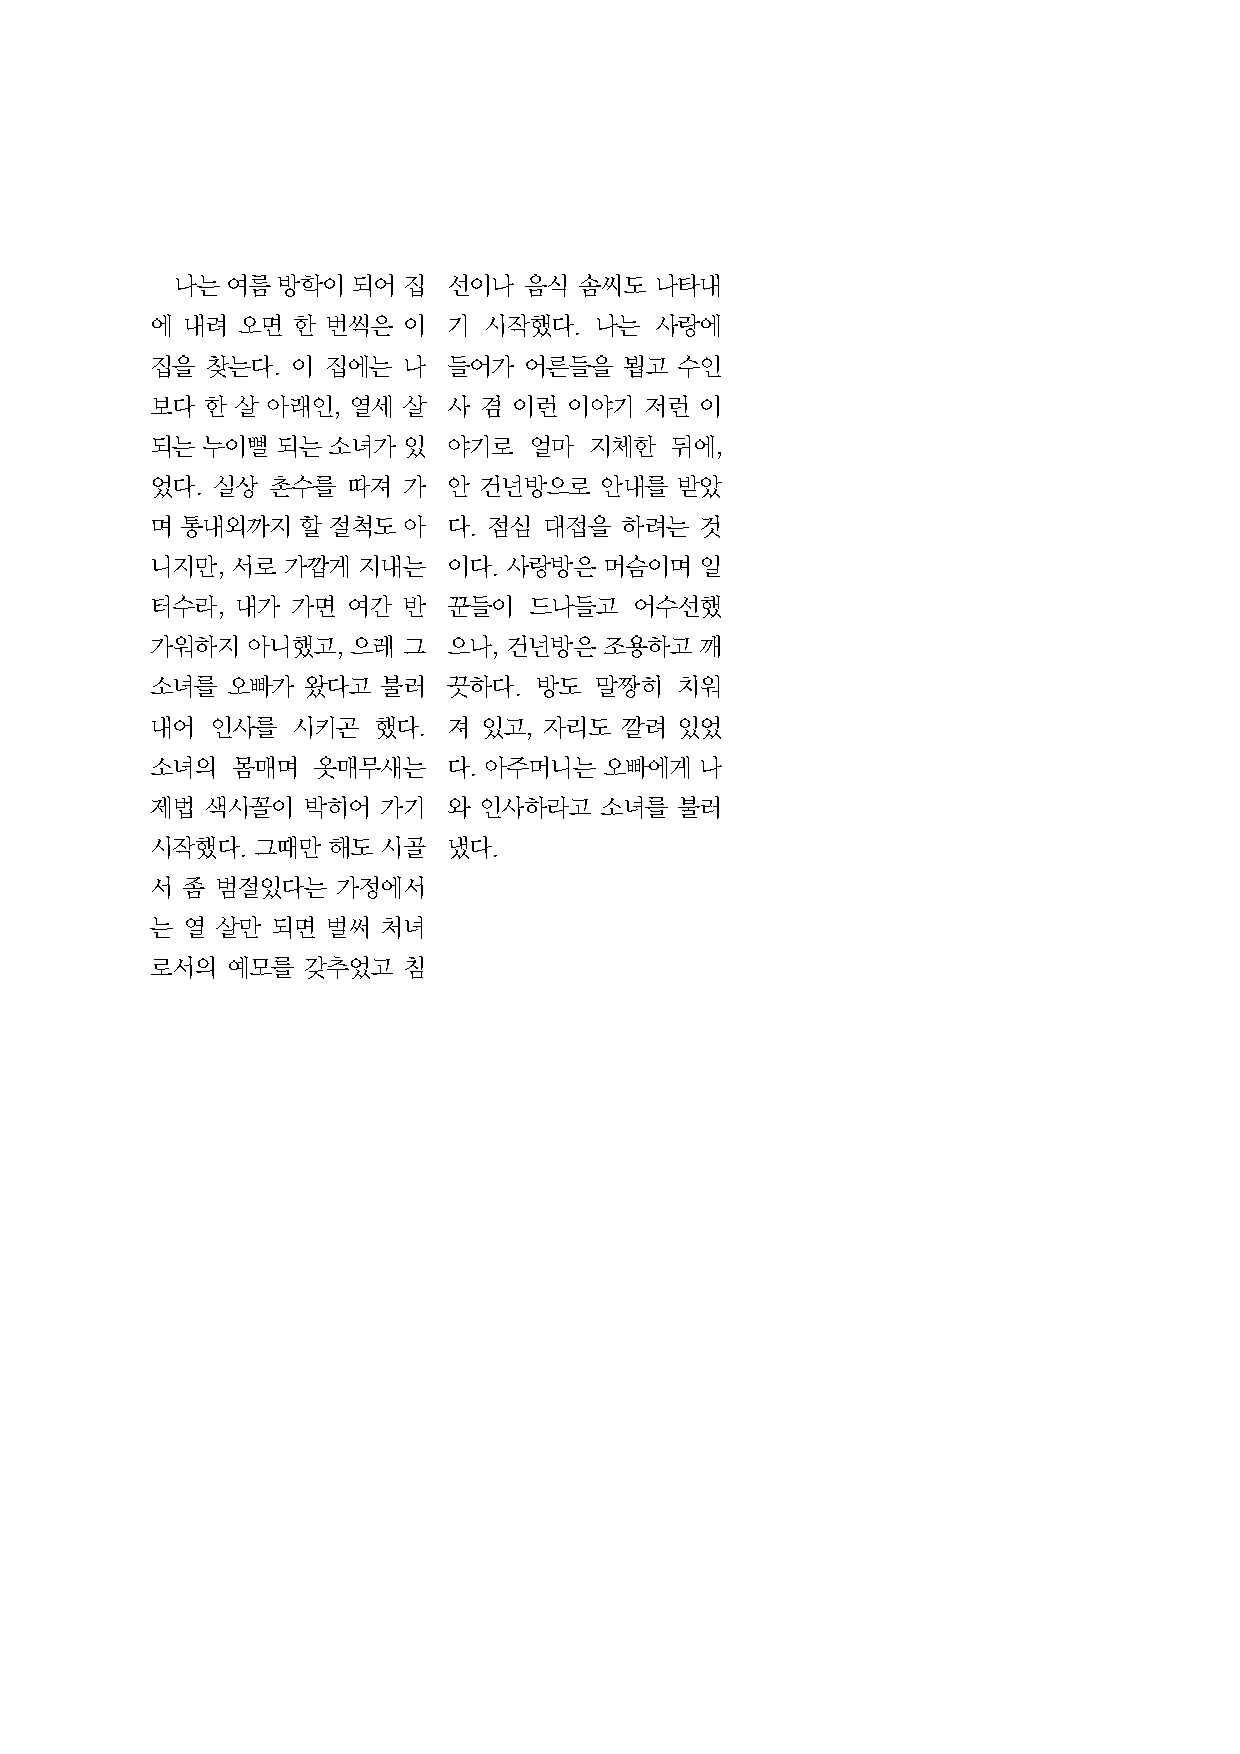
\includegraphics[width=.48\textwidth]{fig/fntnormal}\hfill
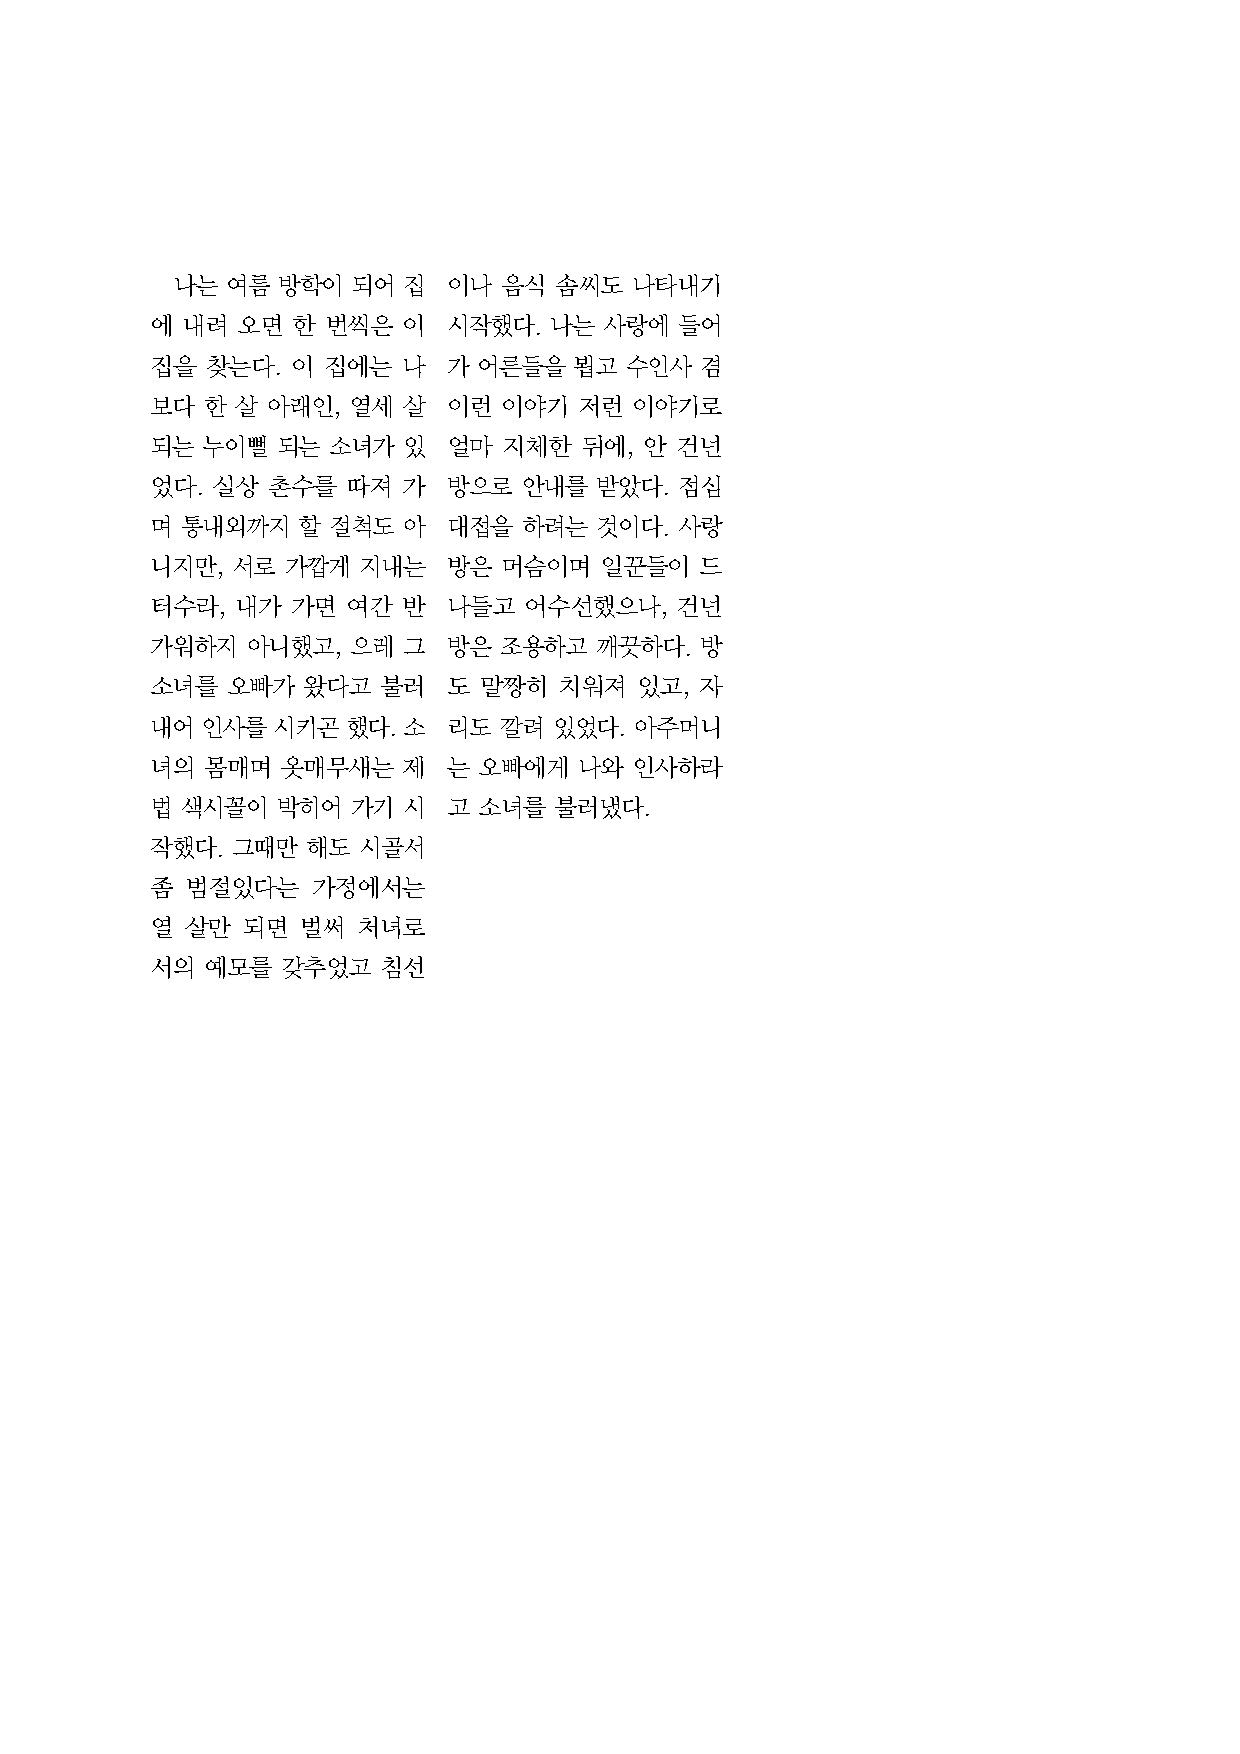
\includegraphics[width=.48\textwidth]{fig/fntexp}\\
\parbox{.48\textwidth}{\centerline{\sffamily\small font expansion 적용 안함}}\hfill
\parbox{.48\textwidth}{\centerline{\sffamily\small font expansion 적용}}
\caption{Font Expansion}\label{fig:fontexpansion}
\end{figure}

샘플 문서의 소스 중에서 font expansion과 관련된 부분은 다음과 같다.
\begin{verbatim}
\usepackage[verbose=true]{microtype}
\DeclareMicrotypeSet{dhucsmicro}{encoding=LUC}
\UseMicrotypeSet[expansion]{dhucsmicro}
\end{verbatim}

\section{행나눔}\index{행나눔}

한글에는 하이픈이 없고 일부 문장부호의 금칙처리를 제외하고는
원칙적으로 모든 문자 앞이나 뒤에서 행을 나눌 수 있다.

\subsection{영문자와 숫자 뒤의 한글 개행}

그림~\ref{fig:allowbreakproblem}에서 표시한 곳은 원본에 영문과 조사가 붙어 있는 부분이다.
빨간색 동그라미 부분에서 영문 단어가 \wi{overfull}이 발생했음에도 불구하고 
뒤에 붙는 한글 조사와 분리되지 않아서 ``\verb|에|''까지 오른쪽으로 
삐져나가 있다. 종래 한글 라텍에서는 이러한 문제가 자주 발생하여
문서작성자를 괴롭히곤 했다.

\begin{figure}
\centering
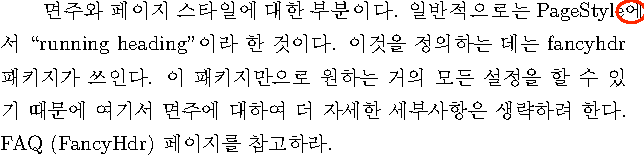
\includegraphics{fig/linebreaktest}
\caption{행나눔 문제}\label{fig:allowbreakproblem}
\end{figure}

\kotex 은 개선된 \wi{행나눔} 기능이 작동한다. 그림~\ref{fig:allowbreakdone}\는
\kotex 을 사용했을 때 이 부분이 어떻게 처리되는가 보여준다.

\begin{figure}
\centering
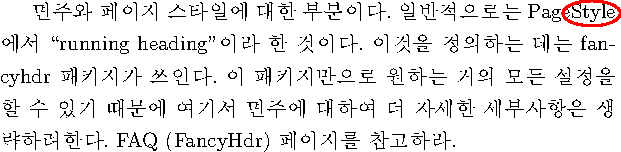
\includegraphics{fig/allowbreak-dhucs}
\caption{dhucs의 행자름 처리}\label{fig:allowbreakdone}
\end{figure}

\subsection{여는 괄호 앞의 행자름}

\wi{여는 괄호}와 관련해서 다음을 지적해둔다. 현재 여는 괄호는 영문자 뒤에 직접
이어서 나오지 않는 한 새로운 줄을 시작할 수 있다. \wi{신정식} 님께서 알려주신 바에
의하면\footnote{\url{http://ktug.kldp.net/jsboard/read.php?table=ktugbd&no=4825}}
모든 종류의 여는 괄호는 새로운 줄을 시작하는 것이 유니코드 표준이라고 한다.
영문으로 글을 쓸 때는 여는 괄호 앞에 하나의 공백을 두게 되어
자연히 새로운 줄을 시작할 수 있을 것이므로 영문자 사이의 여는 괄호를
개행가능하게 하여야 할 필요를 발견하지 못하였다. 그러나 한글과 영문이
만나는 곳에서는 행나눔이 가능하여야 한다. 그림~\ref{fig:openingparen}\을
보라.

\begin{figure}
\centering
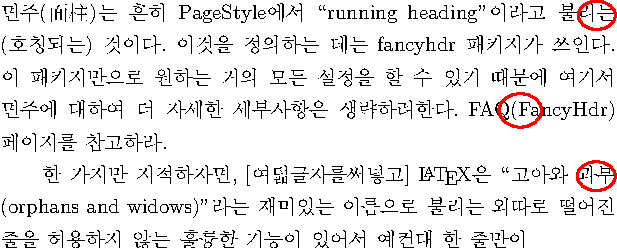
\includegraphics{fig/testdhucsallowbreak}
\caption{여는 괄호의 행자름}\label{fig:openingparen}
\end{figure}

만약 이 그림에서 ``FAQ(FancyHdr)''의 괄호 사이에서 행을 잘라야 한다면
여는 괄호 앞에 공백을 두어
\verb*|FAQ (FancyHdr)|와 같이 써야 할 것이다.

이밖에, \kotex 은 한글 단어 뒤에 괄호 안에 영문을
병기하는 경우 이 영문이 행끝에 걸리더라도 영문 하이픈처리가 작동하도록
하고 있다.

\subsection{이른바 ``고아'' 문제}

``고아''란 한 문단의 마지막 행이 한 글자와 종지부호로만 끝나는 경우를
일컫는다. 한 행 전체 길이에 비교해보았을 때 한 글자 한 행은 그 비중이
너무 작아서 때때로 글읽기의 효율을 방해하고 불필요한 공백이 생겨나게 하여
판면의 색조를 옅게 만드는 것으로 생각되어, 일찍부터 한글 조판의
금기 사항 중 하나였다.\footnote{%
  영어권에서 `고아와 과부'라고 할 때는 이와 조금 다른 의미로 쓰이는
  경우도 있다. 예컨대 Peter Wilson의 \textit{Memoir Manual}, p.~29에는
  ``\emph{고아}란 한 페이지의 마지막에 한 줄 또는 두 줄이 남는 것을 말한다. 
  Bringhurst의 암기를 위한 트릭에 따르면,
  `고아는 미래만이 있고 과거가 없는 것'이다.''라고 쓰고 있다.
  즉, 과부와 고아가 모두 행나눔에 관한 문제가 아니라
  페이지 나눔에 관한 문제로 취급되고 있는 것이다. 그러나
  이 글에서는 우리나라의 관행적 명칭인 `문단 끝 한 글자 한 행'을 (편의상)
  고아라고 부르기로 한다. 
}

\kotex 에서는 고아 회피가 부분적으로 자동화되었다. 원칙적으로
문단 마지막에 아무런 추가 코드 없이 \verb|\par| 또는 문단 종지 문자가
있을 때는 고아 앞에서 \verb|\nobreak|가 작동하는 것과 같은 효과를
가진다. 그러나 문단 끝에 추가적인 코드나 문자가 더 있을 때 때때로
이 자동 고아 회피가 동작하지 않는 경우도 있으므로, 이럴 때는 
\texttt{\textbackslash nobreak}를
사용자가 직접 지정하여야 한다. 특히 문단의 마지막 글자가 ``다.''일 경우에
한하여 사용자가 고아 회피를 강제하도록 ``\verb|\다|'' 매크로가
새로 도입되었다.
%\footnote{%
%  \url{http://kts.ktug.kr/node/204}.
%}
각주 안과 같이 문단 종지 문자 없이 문단이 종료됨으로써
자동 \wi{고아 회피}가 동작하지 않는 경우에
이 매크로를 적절하게 활용할 수 있다.

비록 모든 경우에 완전한 고아 회피가 적용되는 것은 아니지만, 
이만큼이라도 자동화됨으로써 한글 문서 조판의 관행적 규약에 더 가까이
접근했다 하겠다.

\section{한글 PDF 만들기}\label{sec:pdf}

%\pageref{sec:makepdf}페이지 \ref{sec:makepdf}절에서
%pdf 제작에 관한 사항을 개괄하였다. 여기서는 이 문제에 대하여
%조금 더 다루려고 한다. 

version 3.0 문서를 읽고 있는 현재, \pdfTeX 이나 \util{dvipdfmx}를
이용하여 한글 pdf를 제작하는 것은 거의 완벽하게 해결되어 있고, 사용자가
별달리 신경쓸 것이 없어졌다.

역사적으로,
한글 pdf 문서를 만드는 데 있어서 지금까지 요청되어 왔던 것은 대략
다음과 같\다.
\begin{itemize}
\item 한글 텍스트의 검색과 추출
\item pdf bookmark에 한글 구현
\item beamer 등 발표 문서 작성 패키지 지원
\end{itemize}

\subsection{하이퍼링크}\label{sec:hyperref}
하이퍼링크를 구현하기 위해서는 \pkg{hyperref}\를 이용한다.
이 패키지 사용에서 주의할 점은 한글 레이블이나 참조자를
사용하면 아니된다는 것이다.\footnote{%
	이것은 명백히 Legacy \TeX 의 제약이다.
	\XeTeX 과 같은 유니코드 텍 시스템에서는 한글 레이블 등을 자유롭게 사용할 수 있다.}

hyperref 설정은 다음 세 가지 방법으로 이루어진다.
\begin{enumerate}
\item\label{itm:one} \verb|\usepackage[...]{hyperref}|의 옵션
\item\label{itm:two} \verb|\hypersetup| 문장
\item\label{itm:three} \file{hyperref.cfg}에 미리 설정된 옵션
\end{enumerate}
%예컨대 한글 문서를 주로 작성하는 경우 hyperref의 \texttt{[unicode]}
%옵션이 필요하다. 그리고 
클래스 자신이 hyperref을 스스로 로드하는
경우에는 (\ref{itm:one})이나 (\ref{itm:two})\과 같은 방법으로
이 옵션을 활성화할 수 없게 되어 있는 경우가 있다. 이럴 때는 (\ref{itm:three})
방법을 사용한다. 즉 \file{hyperref.cfg}에 (\ref{itm:two})의 문장을
미리 적어넣어두는 것이다.


%\subsection{한글 책갈피}\index{pdf bookmark}
%pdf 문서 제작에 있어서 한글 책갈피(bookmark)가 필요하면,
%다음과 같이 한다.
%\begin{verbatim}
%\usepackage[pdfencoding=auto,<driver>,...]{hyperref}
%\end{verbatim}
%\pkg{hyperref}의 개선이 이루어짐에 따라, 한글 책갈피를 만들기 위해
%별도의 복잡한 조치를 취할 필요가 없게 되었다. 
%%다만, 컴파일 루트에 따라서 \verb|<driver>|를
%%명시해주어야 한다는 데 주의하면 된다. \verb|pdftex|, \verb|dvipdfm|,
%%\verb|dvips| 등을 지정한다.\footnote{\XeTeX, \LuaTeX에서는 \texttt{<driver>}를 별도로 명시할 필요가 없다.}
%

\section{찾아보기와 참고문헌}

\wi{색인}(찾아보기, index)을 만들기 위해 제공하는 유틸리티
\util{komkindex}의 사용법에 대해서는 \pageref{sec:komkindex}
페이지 \ref{sec:komkindex}절을 보라. %이 유틸리티와 더불어
한글 색인 스타일인 \verb|kotex.ist|를 제공한다.

\wi{문헌목록} 인용은 가능하다. Bib\TeX\ 또는 \util{biber}\을 이용하여
문헌목록 데이터베이스에서 문헌목록을 추출할 수도 있다.\footnote{%
  다만, 한글화된 문헌목록 스타일이 충분하지 않아서,
  최종적으로 약간의 수작업이 필요한 경우도 없지는 않다고 생각한다.
  특히 저자-연도 방식의 인용에서 그러하다. 이 분야는
  더 많은 연구와 개발이 필요한 지점이다.}

%여기서는 plain 형식의 인용을 테스트해보자.
%즉, \cite{dhhangul} 또는 \cite{yeonam}\과 같은 형식의 문헌 인용이
%가능한 것을 볼 수 있다.

%\begin{quote}
%\cite{dhhangul}\을 보라. \cite{karnes}\를 읽어보라.
%\end{quote}

\wi{참고문헌} 인용은 너무나 많은 유형이 있어서 어떤
문제가 발생할 수 있는지를 완전히 시험해보지 못하였다.
그러나 \pkg{natbib}, \pkg{cite}와 \pkg{apacite}를 위한
코드를 내장하고 있어, 참고문헌 인용에서 발생하는 문제에 대한
지원을 위해 노력하고 있다.\footnote{%
  한 예로, \pkg{apacite} 충돌 문제의 보고와 그 해결에 관한
  \href{http://ktug.kldp.net/jsboard/read.php?table=operate&no=21183}{KTUG 게시판 4984}
  이하의 글타래를 참조하라. 이런 과정을 거쳐서 현재
  \pkg{apacite} 등의 패키지에 대한 지원이 이루어지게 되었다.}

최근 주목받고 있는 \pkg{biblatex}을 이용하면 한글 문헌목록을
더 잘 작성할 수 있다는 보고가 있다. 이 분야에 대해서 더 깊은
연구가 필요하다.

\section{옛한글 구현}\index{옛한글}

옛한글 문서의 조판은 한글 \TeX 의 꿈이었고, KTUG에서 2002년 이후
\pkg{dhhangul}과 같은 Lambda 패키지를 통하여 성공적인 실험을 행한 바가
있다.

pdf\LaTeX 으로 조판하는 상황에서,
(비록 CTAN에 업로드되지는 않았지만) KTUG 사설저장소를 통하여 배포하는
\pkg{dhucs-midkor}\는 옛한글, 즉 1933년 이전 표기법 문헌을
식자할 수 있게 한다.\footnote{%
	현재 이 패키지를 사용 가능하게 하려면 \cmd{tlmgr install kotex-midkor}
	명령을 \kotex\ 저장소를 등록한 후에 내려야 한다.
	dhucs-midkor는 \kotex-utf의 일부이지만, 몇 가지 이유(주로 글꼴 관련된) 때문에
	별도의 패키지로 분리되어 있다.}
필요한 것은 이 패키지를 설치한 후에 옛한글 텍스트를 이른바 ``첫가끝'' 방식으로
입력하는 것뿐이다.\footnote{%
	``첫가끝(LVT)'' 방식으로 입력한다는 것은 유니코드 자모 조합형으로 한글을
	입력한다는 뜻이다. 예컨대 `가'라는 글자는 \textsf{[U+AC00]}에 완성형 문자가
	있는데, 이 음절 영역 완성형 코드를 사용하지 않고 자모 영역의 초성 `ㄱ'과 중성 `ㅏ'를 결합하여 \textsf{[U+1100][U+1161]}로 조합하여
	표현하는 것을 말한다. 이런 식의 자모 조합으로 한글을 표현하면
	그 표현 한계에 제약이 거의 없으며 현대 한글과 옛한글 수백만 자를 모두 표현할 수 있다.
}
%그러나 배포판의 매크로만으로 충분하지 않으며,
%다음과 같은 준비가 더 필요하다.
%\begin{enumerate}
%\item 옛한글 폰트(\file{obatang.ttf} 또는 \file{ogulim.ttf})
%\item 옛한글 코드 변환 유틸리티
%\item 옛한글 코드를 다룰 수 있는 편집기와 입력기
%\end{enumerate}

이전에는 옛한글 문헌의 조판이 꽤 까다롭고 복잡한 일이었으며,
그런 상황에서 \kotex 이 옛한글 조판 능력을 갖추고 있다는 것은 매우
중요한 일이었다. 현재로서도 그 성취를 가볍게 볼 수는 없으나, 전에 비하여
옛한글을 포함하는 고문헌 조판이 매우 용이해진 것도 사실이다.
\begin{enumerate}[(1)]
\item 옛한글 처리 기능을 갖춘 글꼴이 다양해졌다. 이 분야에서 KTUG의
은바탕 글꼴은 단연 선구적인 위치를 차지하고 있으며, 실무에 쓸 수 있을 정도의
품위를 갖춘 ``함초롬 LVT'' 글꼴의 등장이 차지하는 의미는 매우 중요하다.
그 후, Windows 8에 번들된 ``맑은 고딕''에 같은 기능이 포함됨으로써,
사실상 옛한글 표현과 관련된 글꼴 문제에 있어서 중요한 진일보를 이룩하게 되었다.\footnote{%
	이와 더불어, 예전 쓰이던 이른바 ``한양 PUA'' 방식은 역사의 뒤안길로
	사라질 때가 되었다고 본다.}
\item 플랫폼을 막론하고 ``첫가끝'' 옛한글을 입력할 수 있는 \wi{한글 입력기}들이 등장하였다.
맥 오에스의 하늘입력기, 구름입력기 등으로 첫가끝 옛한글을 손쉽게 입력할 수 있게 되었으며 윈도우즈에도 새나루 입력기와 같이 이를 가능하게 하는 것들이 있다. 
\item \kotex 의 중요한 기여 중의 하나인 옛한글 관련 코드변환 유틸리티가 
\kotex-utility로 제공된다. \util{jamo-normalize} 스크립트는 특히 유용하다.
\item \XeTeX-\ko와 \LuaTeX-\ko는 옛한글 처리 기능을 자연스럽게 탑재하고 있다. 
옛한글을 마치 현대한글을 쓰듯이 자연스럽게 처리할 수 있는 것이다. 이 현대적
텍엔진을 이용하는 것이 현재 권장하는 바이다.
\end{enumerate}
%을 위해서 갖추어야 할
%조건이 제법 까다롭고
%\footnote{%
%  특히 옛한글을 처리할 수 있는 공개 폰트가 전혀 없다는 점은
%  매우 치명적이다.}
%이를 처리하는 과정이 편리하다고 할 수 없다%
%\footnote{%
%  코드 변환과 같은 약간의 전처리가 필요하다.}%
%고는 하나, 
%옛한글 문헌의 식자를 구현하고 있다는 자체가 매우 중요한 사실이다.
%옛한글 조판에 관한 전반적인 사항, 이론적 배경과 구체적인 지침은 \cite{LeeKH}\을
%참고하라.

다음 송강의 \cnm{사미인곡} 예문은 위키문헌에서\footnote{%
	\url{http://ko.wikisource.org/wiki/\%EC\%82\%AC\%EB\%AF\%B8\%EC\%9D\%B8\%EA\%B3\%A1}}
가져온 텍스트를
다음과 같은 명령을 주어 전부 첫가끝 코드로 바꾸고 \pkg{dhucs-midkor} 
패키지를 얹은 후에 (별다른 조치 없이) 그대로 포함한 것이다. 이 유틸리티의
사용법은 \pageref{sec:hypuautil}페이지 \Cref{sec:hypuautil}을
참고하라.
\begin{verbatim}
# jamo-normalize -d -o <yettest.txt >yettest.tex
\end{verbatim}
만약 현대한글까지 전부 첫가끝으로 바꾸지 않으면 현대한글 음절문자가
본문의 것과 똑같은 모양으로 찍힌다.

%\begin{verse} 
%\ifPDFTeX\def\mymidkorfont{ogul} % or {obat}
%\else\ifLuaOrXeTeX \hangulfontspec[Script=Hangul]{HCR Dotum LVT}\fi\fi
%\IfFileExists{yettext.tex}{\input yettext}{}
%\end{verse}
\bigskip
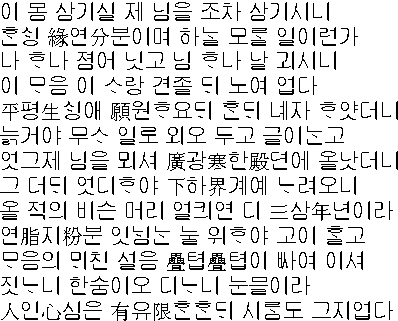
\includegraphics{fig/yettext}

\medskip

\pkg{dhucs-midkor}로 옛한글을 표현할 때 선택할 수 있는 글꼴은
바탕체와 굴림체 두 가지이다. 위의 예문은 굴림체로 식자되었고 이것이 디폴트이다.
만약 바탕체로 식자하려면 \verb|\def\mymidkorfont{obat}|라고
선언하면 된다. 그런데 obatang이라는 글꼴에서 온 바탕체 옛한글은
굴림체에 비해 그다지 예쁘지 않다.

일반적인 의미에서 본격적인 옛한글 문서를 작성하려 한다면
\kotex-utf보다는 \XeTeX-\ko가 더욱 적절하다.
이 새로운 엔진을 기반으로 한 \kotex\ 패키지들은 옛한글에 대한 거의
모든 문제를 완벽하게 해결해두고 있다.

\section{일본어와 중국어 문단}\index{일본어 문단}

\kotex 에는 \pkg{dhucs-trivcj}가 포함되어 있다.
이것은 한글 문서에서 약간의 \wi{일본어} 또는 \wi{중국어} 인용문을 처리하게 하려는
목적으로 제작된 것으로서 본격적인 \wi{다국어 문서}를 처리하는 데는 아직
미흡하지만 크지 않은 규모의 일본어 중국어 문단은 나쁘지 않은 정도의
결과를 얻을 수 있을 것으로 생각하고 있다.\footnote{%
	\pkg{xetex-ko}, \pkg{luatex-ko}에서는 별도의 패키지를
	로드하지 않아도 \texttt{\textbackslash japanese} 명령을
	쓸 수 있다. 특히 \pkg{luatex-ko}는 자체에 ruby 기능을 가지고 있다.}
일본어 한자의 독음을 작은 가나 문자로 붙이는 것(루비)은 \pkg{CJK}의
일부인 \pkg{ruby}\를 불러서 할 수 있다.\index{루비}\footnote{\pkg{CJK}의
\pkg{ruby}가 가진 몇 가지 문제점 때문에 \pkg{ksruby}라는 별도의
패키지를 KTUG 사설저장소에서 제공한다. 루비가 중요한 문서라면 이
패키지를 고려해볼 수 있다.}
일본어 또는 중국어 문단을 식자하려면 \pkg{dhucs-trivcj}를
로드하여야 한다.

%\begin{japanesechinese}

\begin{quote}
\begin{japanese}
\LaTeX~というのは、市販ソフト顏負けのきれいな文書が
作れる「文書整形ソフト」で、「ラテック」
もしくは「ラテフ」など変った読み方をします。
ちょっとカタい言葉を使うと「\ruby{組版}{くみはん} ソフト」とも言います。
組版とは、活字を組んでページに印刷するための版を作る作業のことで英語で
タイプセッティング~(type setting)~と言います。
\end{japanese}
\end{quote}

일본어와 중국어 글꼴은 \TeX{}Live에 기본으로 포함되어 있는
wadalab-unicode 글꼴과 arphic 글꼴(type 1)을 이용한다. 
\TeX{}Live를 full로 설치하면 당연히 시스템에 설치되어 있을 것이므로
별도의 글꼴 설치 절차 없이 바로 이용할 수 있다.
다만 이 글꼴에는
굵은글꼴이나 고딕체 글꼴이 별도로 갖추어져 있지 않다.
일본 문자와 로마자가 이어질 때 필요한 `\wi{짧은 간격}'은 tilde(\verb|~|)로 표시할 수 있다.
이것은 \pkg{CJK}의 방식과 동일하다.

\pkg{dhucs-trivcj}가 제공하는 환경은 \texttt{japanese}와
\texttt{chinese}이다. 다만 \texttt{chinese} 환경은 간자체 환경과
번자체 환경을 각각 \texttt{Schinese}와 \texttt{Tchinese}로
구분할 수 있다. 기본값은 \texttt{chinese}가 간자체 환경으로
되어 있지만 만약 번자체 환경을 \texttt{chinese}로 쓰고 싶다면
\begin{verbatim}
\let\chinese\Tchinese
\let\endchinese\endTchinese
\end{verbatim}
라고 선언하면 된다. 다른 문서와의 호환을 위해서 번자체 환경을
그대로 \texttt{Tchinese}라고 쓰는 것도 좋은 방법이다.

다음 표는 \texttt{dhucs-trivcj}에서 사용하는 각 언어별
폰트의 이름이다. 
\begin{center}
\begin{tabular}{l|ll|ll}
\hline
 & \multicolumn{2}{l|}{trivcj} & \multicolumn{2}{l}{trivcj-adobe} \\
\cline{2-5}
 & mj & gt & mj & gt \\
\hline
일본어 & min & -- & jpmj & jpgt \\
중국어간자 & gbsn & -- & cnmj & cngt \\
중국어번자 & bsmi & -- & ctmt & -- \\
\hline
\end{tabular}
\end{center}

간단한 중국어 문장 하나를 식자해보자.\footnote{\url{http://wikka.ctex.org/TeX} 웹사이트에서
인용함.}

\begin{chinese}
\begin{description}
\item[{[}高质量的输出{]}] TeX~遵循传统的排版规则,以排版的质量为最重要的目标。
   如果你把~TeX~的输出结果和用其它的排版软件排版相同的文本所得到的结果加以比较,
   你就会发现其中的区别。
    
\item[{[}超常的稳定性{]}] 自从~TeX~出现以来,只有一些微小的改动。也就是说,
  十几年前的~TeX~文件用现在的~TeX~系统排版得到的结果与十几年前得到的结果是一样的。
  稳定性还体现在~TeX~系统极少会崩溃,可以处理任意大小的文件,即使你的计算机的内存很少,
  TeX~也可自如的工作。
\end{description}
\end{chinese}

%\end{japanesechinese}

\section{세로쓰기}

\kotex-utf는 한글 \wi{세로쓰기}를 직접 지원하지 않는다.
몇 가지 편법을 써서 세로쓰기 문단이나 문서를 만드는 실험이 행해진 적이 있지만
일반화할 만한 것은 아니었다.
한편, \XeTeX-\ko는 한글의 세로쓰기가 구현되어 있다. \pkg{xetexko-vertical} 패키지를 이용하여 세로쓰기를 가능하게 한다.

\chapter{글꼴 문제}\index{글꼴 문제}

\XeTeX 이나 \LuaTeX 의 등장으로 가장 급격한 변화를 맞은 것이
한글 글꼴(폰트)의 사용 방식에 대한 것이다. 트루타입과 오픈타입을
직접 사용할 수 있는 이러한 텍 엔진의 등장은 매우 중요하고 극적인 변화를
한글 텍 환경에 도입하게 하였다.
이러한 새로운 텍 엔진에서 폰트를 사용하는 문제는 해당 문서를 참고하라.

이 글은 레거시 텍에서 구현되는 \pkg{kotex-utf}에 관한 것이다.
따라서 이 장 전체의 내용은 오직 \util{latex}이나 \util{pdflatex}으로 컴파일하는 경우에만 해당하며, \XeTeX, \LuaTeX에서 한글을 사용하는 경우와 호환성이 없다.

\section{개관}

현재 버전의 \kotex 은 디자인상 `\wi{기본 글꼴}'이 없다. 이전 버전까지 은글꼴 type 1 (\pkg{untype1})\index{은글꼴 type 1}을 기본 글꼴로 삼고 있었으므로 크게 달라진 점이다.
그런데, 기본 글꼴이 없다는 것은 \cmd{\usepackage\{kotex\}}만으로는
한글 글자가 찍히지 않는다는 것을 의미한다. 실제로 \XeTeX-\ko와 \LuaTeX-\ko는 이런 식으로 동작하고 있으며, 반드시 한글 글꼴을 명시적으로 지정해주어야 하게 되어 있다.

하위 호환성도 염두에 두고 있는 \kotex-utf에서 만약 이렇게 되면 사용자의 혼선을
불러올 것이 자명하므로, 우선 아무런 글꼴도 지정하지 않으면 \pkg{nanumtype1} 글꼴을 불러 글자를 보여주게 되어 있다.\footnote{단, 한자 영역은 \pkg{uhc}.} nanum type 1이 선택된 이유는 이 글꼴 패키지가 CTAN에 등록되어 있고 \TeX\,Live에서 제공하는 것이기 때문이다.\footnote{%
	원래 \pkg{cjk-ko}에서 사용하기 위해 제작된 글꼴이다.}
\index{나눔 type 1}

그러나 이것은 `기본 글꼴'과는 성질이 다른데, 그 이유는 \kotex 이 제공하는
글꼴 처리 능력에 비추어 많은 부분이 생략되어 있기 때문이다. 예를 들면 \texttt{ttfamily}에 해당하는 타자체가 별도로 없다는 점, 한자는 한 가지 글꼴밖에 사용하지 않고 굵은 한자가 찍히지 않는다는 점 등에서 그러하다.

글꼴의 선택과 사용이 전적으로 사용자에게 맡겨져 있으나, ``편의를 위하여''  상세한 글꼴 설정이 없을 때
나눔 type 1이 한글 영역을 식자하기 위하여 사용된다고 기억해두자.

2021년 현재, nanumtype1은 \TeX\,Live를 통하여 설치되기 때문에 거의 유일한
\koTeX-utf 용 글꼴이 되어 있다. 한편, 은 글꼴 type 1은 한글 텍 사용자 그룹이
별도로 운영하는 KTUG 사설 저장소를 통하여 이를 설치할 수 있다.

이보다 더 많은 글꼴을 레거시 텍에서 활용하려면 \pageref{cha:truetype} 페이지의 제~\ref{cha:truetype}~절을
참고할 수는 있지만, \XeTeX 이나 \LuaTeX 으로 트루타입을 직접 활용할 수 있는 오늘날 
이 방법은 낡은 것이 되었다.

\section{영역, 가족, \cntrdots}

\subsection{입력 문자의 영역}

텍스트의 문자를 식자할 때, \kotex 은 입력 문자를 세 영역으로 나누고 각각에
대하여 다른 글꼴을 적용한다.\index{입력문자의 영역}
\begin{enumerate}
\item \textbf{라틴 문자 영역}. ASCII 문자들은 모두 여기에 들어간다. 즉
로마자 알파벳과 숫자, 일부 문장부호들이다. 
이 영역의 문자를 식자하는 것은 일반적인 라틴 문자 문서와 완전히 동일하다.
그러므로 \pkg{fontenc}로 OT1, T1 등의 폰트 인코딩을 지정하거나
\pkg{lmodern}, \pkg{txfonts}와 같은글꼴 패키지를 사용하는 것도
이 영역에 영향을 미친다.\index{라틴문자 영역}

\item \textbf{한글 영역}. [U+AC00]에서 [U+D7FF]까지 한글 음절문자 영역의
글자와 한글 자모 및 한글 호환자모 글자들에 해당한다. 이 영역을 식자하는 글꼴을
`한글 글꼴'이라 한다.\index{한글 영역}

\item \textbf{한자 영역}. 위의 라틴 문자 영역과 한글 영역을 제외한 모든
문자가 포함된다. 한중일 호환 문장부호, 한자는 물론이고 일부 폰트에서
발견할 수 있는 PUA(사용자 영역) 옛한글 문자도 여기에 속한다. 이 영역은 `한자 글꼴'로 식자한다.\index{한자 영역}
\end{enumerate}
이 세 영역은 완전히 분리되어 있고 서로 영향을 미치지 않는다. 즉
한글 영역의 글꼴을 바꾸더라도 라틴문자나 한자 영역의 글꼴의 선택이
(원칙적으로) 바뀌지 않는다. 

\subsection{라틴 문자 영역 글꼴}

\thispkg의 라틴 문자 글꼴 기본값은 OT1 인코딩의 \wi{CM}이다.
\wi{T1 인코딩}으로 \wi{EC 글꼴}을 사용하려면 다음을
전처리부(preamble)에 적어준다.
\begin{verbatim}
\usepackage[T1]{fontenc}
\end{verbatim}
글꼴 설정 패키지를 사용하면 이 영역 문자에 영향을 미친다.
예를 들어 \wi{pxfonts}를 본문에서 쓰려면,
\begin{verbatim}
\usepackage{pxfonts}
\end{verbatim}
와 같이 한다.

NFSS\footnote{\LaTeX 의 폰트 선택 스킴을 가리킨다.}를 따르며, rm, sf, tt
패밀리와 md, bf 시리즈, up, it, sl 셰이프들을 선택하는 폰트 선택 명령 역시
그대로 적용된다.

\pkg{kotex} 자체가 font encoding을 정의하고 있기 때문에, font encoding을 바꾸는
명령, 예를 들면 \verb|\usepackage[T1]{fontenc}|과 같은 행은 \pkg{kotex}이
로드되기 전에 부르는 것이 좋다.

이후의 논의는 한글 및 한자 영역 글꼴에 관한 사항이다.

\subsection{글꼴 가족과 인코딩}

\kotex 은 한글과 한자 영역 글꼴에 대해서도 \wi{NFSS} 방식의
글꼴 선택이 동작하도록 설계되어 있다.\index{글꼴 가족}

이 영역 글꼴을 rm, sf, tt 세 글꼴 가족(family)으로 구분한다.
각각을 편의상의 명칭인 ``바탕(또는 명조), 돋움(또는 고딕), 타자''에
대응시킨다. 이들은 라틴 문자의 ``serif, sans serif, typewriter''에
해당하는 것으로 본다.

\begin{center}
\begin{tabular}{c|c|c|c}
\hline
 & rm & sf & tt \\ \hline
한글 & 한글바탕글꼴 & 한글돋움글꼴 & 한글타자글꼴 \\ \hline
한자 & 한자바탕글꼴 & 한자돋움글꼴 & 한자타자글꼴 \\ \hline
\end{tabular}
\end{center}

\kotex 이 한글과 한자 영역 식자에 사용하는 폰트는 LUC 인코딩
폰트이다. 이 인코딩은 유니코드 문자군을 수백 개의 subfont로 분할하여
처리하도록 되어 있어 실제 글꼴 파일 자체의 구성은 매우 복잡하지만 \TeX 의 
폰트 정의 (font definition) 방식에 의하여 대표 이름으로 호출할 수 있다.

다른 글꼴 선택 없이 나눔 type 1으로 식자하는 경우, 이 글꼴가족들은 다음과 같이 대응되어 있다. 
타자체 글꼴을 별도로 할당하지 못한 것은 해당하는 글꼴이 없기 때문이다. 참고로
은글꼴 type 1을 쓴다면 uttz라는 은타자 글꼴을 이 영역에 할당할 수 있었다.\footnote{%
	은타자 서체를 타자체 패밀리로 지정하는 방법은 \pageref{sec:oldmethod}페이지를
	보라.}

\begin{center}
\begin{tabular}{c|c|c|c}
\hline
 & rm & sf & tt \\ \hline
한글 & nanummj & nanumgt & nanumgt \\ \hline
한자 & uhcmj & nanumgt & nanumgt \\ \hline
\end{tabular}
\end{center}

글꼴 가족을 지정하는 것은 다음 NFSS 명령을 쓴다. 
윗줄의 세 개는 인자를 갖는 `명령형'이고 아랫줄의 세 개는
`선언형'이다.
\begin{boxedverbatim}
\textrm, \textsf, \texttt
\rmfamily, \sffamly, \ttfamily
\end{boxedverbatim}
이 명령이 주어지면 라틴문자 영역뿐 아니라 한글과 한자 영역에 대해서도
위의 표에 주어진 대응에 따라 한글과 한자를 식자한다.

이밖에 series, shape, size 등에 해당하는 NFSS 명령이
한글과 한자에 다 적용된다.

\kotex-utf에서는 (\XeTeX-\ko와 달리) 수학 문자에
한글 글꼴을 쓸 수 없다. 수학 글꼴들은 라틴 문자와 같이 취급되며
NFSS의 수학 글꼴 명령을 그대로 따른다.
수식 안에 한글 텍스트를 넣어야 한다면 \pkg{amsmath}의
\cmd{\text} 명령을 쓴다.

\section{글꼴의 제한과 더 많은 글꼴 사용에 대한 문제}

Legacy \TeX 과 \XeTeX, \LuaTeX 의 가장 큰 차이 중의 하나가
폰트 문제에 관련된 것이다. 즉 새로운 텍 엔진들은 트루타입, 오픈타입과
같은 글꼴을 자유롭게 다룰 수 있게 됨으로써, 종래 \TeX 의
폰트 사용 방식에 더이상 구애되지 않아도 되게 되었다.

\begin{table}[b]
\centering
\caption{한글 글꼴 사용 범위}
\begin{tabular}{c|c|c|c|c}
\hline
 & mf & type 1 & truetype & opentype \\ \hline \hline
tex + dvips & 가능 & 가능 & & \\ \hline
tex + dvipdfmx & 가능 & 가능 & (변환필요) & (변환필요) \\ \hline
pdftex & 가능 & 가능 & (변환필요) & (변환필요) \\ \hline \hline
xetex & 가능 & 가능 & 직접 사용 & 직접 사용 \\ \hline
luatex & 가능 & 가능 & 직접 사용 & 직접 사용 \\ 
\hline
\end{tabular}
\end{table}

만약 더 많은 글꼴의 사용을 원한다면 이 텍 엔진으로 갈아타는 것이 좋다.
\circemph{폰트가 문제라면 \XeTeX 을 쓰시라.}

애초부터 \kotex 은 폰트 사용에 관하여 많은 
고민이 있었고 몇 가지 방법을 제시한 바 있으며 그 명령들은 여전히 
유효하지만, 굳이 그렇게까지 하면서 Legacy \TeX 에서 ``많은 폰트''를
사용할 필요가 없어졌다.

\subsection{\kotex 의 글꼴 관련 명령}\label{sec:oldmethod}

아래 \kotex 이 마련해 둔 폰트 관련 명령 몇 개를 정리하여 둔다.

\begin{boxedverbatim}
\SetHangulFonts{mj}{gt}{tz}
\SetHanjaFonts{mj}{gt}{tz}
\end{boxedverbatim}
기본 글꼴을 설정한다. 세 개의 인자는 각각 명조/고딕/타자에 해당한다.

\begin{boxedverbatim}
\SetSerifFonts{hangul}{hanja}
\SetSansFonts{hangul}{hanja}
\SetMonoFonts{hangul}{hanja}
\end{boxedverbatim}
두 개의 인자는 각각 한글 영역과 한자 영역을 식자할 글꼴 이름이 온다.

\begin{boxedverbatim}
\SetAdhocFonts{hangul}{hanja}
\end{boxedverbatim}
본문에서 일시적으로 글꼴을 바꾸고자 할 때 쓰기 위해 마련된 명령이다.
특히 이 명령은 한글과 한자 영역에만 영향을 끼치므로 라틴 문자 영역은 별도로
지정해주어야 한다.

\subsection{Legacy \TeX 을 위한 한글 글꼴 패키지들}

새로운 텍 엔진의 등장으로 이제 사실상 필요가 사라졌지만
한때 다양한 글꼴 패키지가 만들어져서 유통된 사례들이 많다.

그 가운데는 백묵 글꼴, 문화부 글꼴, 윈도우즈 기본 글꼴, 한겨레결체 등을
텍이 사용할 수 있도록 조성하여 제공한 경우도 있었으나, 현재 이 패키지들을
찾아보기는 어렵다.

\paragraph{은글꼴 type 1}
현재 \kotex\ 저장소에서 \pkg{kotex-base}라는 이름으로 제공되는
untype1\index{은글꼴 type 1}은 종래 기본 글꼴로 사용되던 것이므로 이 글꼴 패키지를 
다시 사용하기를 원하는 경우가 있을 수 있다.
이 때는 먼저 이 패키지를 
\begin{verbatim}
tlmgr install kotex-base
\end{verbatim}
설치한 후에, 본문에서 다음 한 줄을 추가해준다.
\begin{boxedverbatim}
\usepackage{dhucs-untype1}
\end{boxedverbatim}

\paragraph{트루타입 글꼴}
이제 필요가 줄었지만, 그래도 트루타입 폰트를 \kotex-utf에서 
사용하려 하며, 폰트 라이선스 등에 대하여
자신이 책임질 수 있고, 약간의 복잡한 설정 작업을
기꺼이 해내려 한다면, \textsf{ttf2kotexfont} 유틸리티를 사용하면
된다. 이 유틸리티의 사용법은 이 문서 말미에 별도의 장으로 마련되어 있다(\pageref{cha:truetype}페이지, \ref{cha:truetype}장).

\subsection{엄격한 문자 체크}

한글 문서 작성 상황은 매우 복잡해서, 현재 사용중인 폰트에 사용자가
표현하고자 하는 모든 문자가 구비되어 있지 않은 경우가 많다. 
은글꼴의  은바탕체만 하더라도 예컨대 한자는 KS X 1001에 해당하는 4888자밖에는
들어 있지 않다.

그런데 \TeX 은 \file{.tfm}이 아예 없다면 에러를 내지만 \file{.tfm}은
있으나 그 \file{.tfm}의 문자 정의에 해당 글자가 없는 경우에는
다만 글자를 식자하지 않고 경고만을 보이고 지나가면서 \file{.log}에 기록하는 것에
그친다. 그 결과 \file{.log}를 세심하게 살피지 않으면 혹 부지불식간에
특정 문자를 식자하지 못하는 결과를 초래하게 된다.

이 때문에 도입된 옵션이 \texttt{[strictcharcheck]}이다.
이 옵션을 활성화하면 \eTeX 의 원시명령을 이용하여 만약 \file{.tfm}은
있는데 특정 문자가 없다면 에러를 발생시키면서 컴파일을 멈추게 한다.
문서 작성자는 이를 통해 현재의 상황을 보다 잘 인식하고 폰트를 교체하거나
임시 폰트를 지정하는 등의 조치를 취할 수 있을 것이\다. \index{strictcharcheck}\index{엄격한 문자 체크}

이 옵션을 지정하지 않으면 에러를 보여주지 않고 다만 \file{.log}에만
기록한다.

\chapter{한글 문서 서식을 위한 부가 패키지들}

이 장에서 설명하는 부가 패키지들은 \pkg{kotex-utf}에서만 활용할 수 있으며
\XeTeX, \LuaTeX을 사용하는 경우와는 호환성이 없다.

\section{강조 방식}\label{sec:gremph}

\ref{sec:emphasis} 소절에서 논의한 바와 같이 강조 명령(\cmd{\emph})이
주어졌을 때 기울인 글자체를 쓸 것인지 글꼴 대체 방식을 쓸 것인지를 정할 수 있게
하는 부가 패키지가 \pkg{dhucs-gremph}이다.

이 패키지를 로드하면 \cmd{\emph} 명령의 강조 부분이 \emph{나눔고딕}으로 식자된다.
은글꼴 type 1 패키지를 사용할 경우, 은그래픽 서체가 기본이었던 것을 상기하라.

패키지가 제공하는 명령이 몇 가지 있다.

\begin{boxedverbatim}
\SetGremphFonts{hangul}{hanja}
\end{boxedverbatim}
강조 부분에 식자할 글꼴을 지정한다.\footnote{%
	현실적으로 생각해보면 현재의 \kotex\ 이용 상황에서
	\pdfLaTeX 으로 사용자가 추가적인 type 1 글꼴이나 트루타입 \TeX\ 글꼴을 사용하게 될 가능성은
	거의 없다고 보는 것이 좋을 것이다. gremph 기능도 결국 글꼴의 문제이므로 이 문제를 더
	섬세하게 제어하려면 \XeTeX\ 엔진을 사용할 것을 권한다.}
주의할 점은 은글꼴이나 \util{ttf2kotexfont}로
설치한 트루타입 글꼴 사용시에는 폰트 이름 앞에 `o'를 하나 붙여주어야 한다는 점이다.
즉
\begin{verbatim}
\SetGremphFonts{nanummj}{nanumgt}
\end{verbatim}
으로 좋지만, 은글꼴일 경우
\begin{verbatim}
\SetGremphFonts{outgr}{outgt}
\end{verbatim}
와 같이 지정해야 정상적으로 동작한다.

\begin{boxedverbatim}
\ungremph, \regremph
\end{boxedverbatim}
강조 방식을 기울인 글꼴로 되돌리거나 이를 다시 글꼴 대체 방식으로 하라는 명령이다.

%만약 emph에 해당하는
%글꼴을 그래픽이 아닌 다른 글꼴로 바꾸고 싶다면 다음과 같이 한다.
%\begin{verbatim}
%\usepackage[gremphhangul=unbm,gremphhanja=unyt]{dhucs-gremph}
%\end{verbatim}
%첫번째 인자는 한글, 두번째 인자는 한자 글꼴을 지정하는 것이다.
%또, emph에 해당하는 문자를 굵은글꼴로 하고 싶으면,
%\begin{verbatim}
%\usepackage[bfemph]{dhucs-gremph}
%\end{verbatim}
%와 같이 \verb|[bfemph]| 옵션을 지정한다.\footnote{%
%	은글꼴 중에는 boldface 글꼴이 따로 마련되어 있지 않은 것이 많다는
%	점에 주의하라. 이 경우에는 약간의 Warning을 내면서 그냥 보통 글꼴로
%	식자된다.}
%문서의 중간에서 기울임 방식과 글꼴 변경 \verb|\emph| 방식을 바꿀 수도 있다.
%각각 \verb|\regremph| 명령과 \verb|\ungremph|를 사용한다. 
%\regremph\verb|\regremph|를 지정한 경우에는,
%\begin{quote}
%\emph{테스트. test.}
%\end{quote}
%와 같이 식자되고, \ungremph\verb|\ungremph|를
%설정한 경우에는, 
%\begin{quote}
%\emph{테스트. test.}
%\end{quote}
%와 같이 식자된다.
%\regremph

\section{각주 형식}\label{sec:fn}

\subsection{dhucsfn의 각주 판짜기}

\pkg{dhucsfn} 패키지는 \wi{은광희}의 H\LaTeX\ 1.0.1과
\kotex-euc에 있는 \pkg{hangulfn} 패키지를 \kotex 으로
포팅한 것이다. 아래 사용법 설명과 용어는 원본 패키지에 대한
설명을 담고 있는 hlatexguide 문서에서 그대로 가져왔다.

\bigskip

패키지의 사용법은 다음과 같다.
\begin{verbatim}
    \usepackage[선택사항]{dhucsfn}
\end{verbatim}

\texttt{선택사항}(옵션)으로는 각주 번호의 판짜기 방식을 지정하는
\texttt{첨자}와 \texttt{괄호}가 있는데 각각 다음과 같이 짜여진다.
\begin{itemize}
\item \texttt{첨자(superscript)}: \xample{$^1$각주문}
\item \texttt{괄호(parenthesis)}: \xample{1) 각주문}
\end{itemize}
\texttt{첨자}의 경우에는 각주 번호와 각주문 사이가 붙고
\texttt{괄호}의 경우에는 소괄호와 각주문 사이에 구분 공간이 있다.
애초값은 \texttt{첨자}이다.

각주 판면의 판짜기를 지정하는 \texttt{선택사항}의 종류는 다음과
같다.
\begin{itemize}

\item \texttt{다항이어쓰기(multipara)}: 연이은 각주가 새 행에서 시작하지 않고 이전
  행의 오른쪽에 나열되며, 새 각주의 넓이가 행의 오른쪽 경계를 넘어 설
  때에 그 각주는 새 행에서 시작한다.  문서 전체가 길이가 짧은 각주로만
  구성될 때에 사용할 수 있는 판짜기 방식이다.

  \xample{\rule{2in}{.4pt}\\
    \footnotesize 12)~첫번째 각주\qquad 13)~두번째 각주\qquad
    14)~세번째 각주\qquad 15)~네번째 각주\linebreak 16)~다섯번째
    각주\qquad 17)~여섯번째 각주\qquad 18)~일곱번째 각주\qquad
    19) 여덟번째 각주 }

\item \texttt{단순이어쓰기(para)}: ``\texttt{다항이어쓰기}''와 같은 방식이나
  한 각주의 넓이가 행의 오른쪽 경계를 넘어 설 때에 경계를 넘어서는
  부분이 줄바꿈에 의해 다음 행으로 넘겨진다는 점이 다르다.

  \xample{\rule{2in}{.4pt}\\
    \footnotesize 12)~첫번째 각주\quad 13)~두번째 각주\quad 14)~세번째
    각주\quad 15)~네번째 각주\quad 16)~다섯번째 각주\quad 17)~여섯번째
    각주\quad 18)~일곱번째 각주\quad 19)~여덟번째 각주}

\item \texttt{내어쓰기(hang)}: 각각의 각주는 새 행에서 시작한다.  각주 번호가
  각주문의 왼쪽으로 내어 써 지고, 각주문의 왼쪽맞춤 위치가 각주문의 첫
  글자의 위치이다.  이 방식이 애초값이다.

  \xample{\rule{2in}{.4pt}\\
    \footnotesize\tabcolsep0pt
    \begin{tabular}[t]{lp{.9\columnwidth}}
    12)~ & 각주면의 각주 번호와 구분 공간을 각주문으로부터 왼쪽으로 내어
    쓰는 방식이다.  각주문의 가로 넓이는 본문의 가로 넓이에서 각주
    번호와 구분 공간의 넓이만큼 뺀 길이이다.
    \end{tabular}
  }

\item \texttt{왼쪽맞춤(leftflush)}: 각각의 각주는 새 행에서 시작한다.  각주의 첫
  줄이 왼쪽맞춤으로 짜진다.

  \xample{\rule{2in}{.4pt}\\
    \footnotesize
    12)~각주 번호와 각주문이 들여쓰기나 내어쓰기에 의해 구분되지 않고
    전체가 하나로 왼쪽맞춤 되는 판짜기 방식이다.  각주 번호와 각주문의
    사이에는 구분 공간이 삽입된다.  구분 공간은 \texttt{첨자}의 경우
    0pt이고 \texttt{괄호}의 경우 공간 문자이다.
  }

\item \texttt{들여쓰기(indent)}: 라텍이 제공하는 기본 각주 판짜기와 유사한
  방식이다.  각주 번호는 3배각의 위치에서 오른쪽으로 정렬되며 각주문이
  구분 공간을 사이에 두고 이어진다.  각주문 사이에 줄바꿈이 일어나면
  새 행이 본문의 왼쪽 맞춤 위치에서 시작한다.

  \xample{\rule{2in}{.4pt}\\
    \footnotesize\settowidth{\dimen0}{각주}
    \hbox to1.5\dimen0{\hss 12)}~첫줄 들여쓰기 방식이다.  각주 번호의
    끝이 왼쪽 가장 자리에서부터 3배각의 위치이다.  연이은 각주의 각주
    번호도 같은 위치에 정렬된다.\\
    \hbox to1.5\dimen0{\hss 13)}~이어지는 각주이다. 각주 번호가 위쪽의
    각주 번호와 함께 오른쪽으로 정렬되었다.
  }

\item \texttt{들여왼쪽맞춤(leftflushindent)}: ``\texttt{왼쪽맞춤}''과 같은 방식이다.
  전체 각주면이 본문으로부터 오른쪽으로 2배각 들여 써진다.

  \xample{\rule{2in}{.4pt}\\
    \footnotesize\settowidth{\dimen0}{각주}\tabcolsep0pt
    \begin{tabular}[t]{lp{.9\columnwidth}}
      \rule{\dimen0}{0pt} &
      12)~각주 번호와 각주문이 들여쓰기나 내어쓰기에 의해 구분되지 않고
      전체가 하나로 왼쪽맞춤 되는 판짜기 방식이다.  전체 각주면이
      본문의 왼쪽맞춤 위치에서 2배각 들여진다.
    \end{tabular}
  }

\item \texttt{들여내어쓰기(hangpar)}: ``\texttt{들여쓰기}''와 같은 방식이다.  전체
  각주면이 본문으로부터 오른쪽으로 2배각 들여 써진다.

  \xample{\rule{2in}{.4pt}\\
    \footnotesize\tabcolsep0pt
    \settowidth{\dimen0}{각주}
    \hspace*{\dimen0}
    \multiply\dimen0 by-1 \advance\dimen0 .89\columnwidth
    \begin{tabular}[t]{lp{\dimen0}}
      12)~ & 각주면의 각주 번호와 구분 공간을 각주문으로부터 왼쪽으로
      내어 쓰는 방식이다.  전체 각주면은 본문의 왼쪽에서 2배각 들여
      짜진다.  각주문의 가로 넓이는 본문의 가로 넓이에서 각주 번호와
      구분 공간의 넓이 그리고 2배각의 넓이를 뺀 길이이다.
    \end{tabular}
  }

\item \texttt{들여괄호맞춤(varhangpar)}:  ``\texttt{들여내어쓰기}'' 방식과 같으나
  각주문에서 줄바꿈에 의해 새로 시작하는 행의 왼쪽이 각주 번호에
  사용되는 괄호의 끝에 정렬되는 점이 다르다.  각주 번호 양식이
  ``\texttt{괄호}''로 바뀐다.  각주 번호와 각주문의 간격은 1배각이다.

  \xample{\rule{2in}{.4pt}\\
    \footnotesize\tabcolsep0pt
    \settowidth{\dimen0}{각주}
    \hspace*{\dimen0}
    \multiply\dimen0 by-1 \advance\dimen0 .89\columnwidth
    \begin{tabular}[t]{lp{\dimen0}}
      12) & ~~각주면의 각주 번호를 각주문으로부터 왼쪽으로 내어 쓰는
      방식이다.  각주 번호와 각주문 사이에는 1배각의 간격이 삽입된다.
      전체 각주면은 본문의 왼쪽에서 2배각 들여 짜진다.  줄바꿈 후에 새
      행이 각주 번호의 괄호 다음에서 시작했다.
    \end{tabular}
  }
\end{itemize}

\subsection{각주 문단 모양 관련}

한글 문서는 기본 행간을 영문 문서에 비하여 넓혀 잡기 때문에 각주 사이의
간격이 흐트러져서 모양이 일그러지는 경우가 생긴다. 즉, 한글 문서에서는
각주 사이의 간격을 적당하게 재조절해주어야 한다. 이에 대해서 \pkg{dhucs-setspace}가 약간의 해결책을
제시해주시만, 각주 내의 행간을 재조절하는 특징이 있다.
일반적인 문서에서 각주 행간을 본문 행간과 동일하게 할 것인가 아니면
좁은 행간을 쓸 것인가는 전적으로 선택의 문제이지만, \verb|\footnotesep|
길이값을 저자가 직접 설정해줄 필요가 있다는 점을 기억해두자. 

\wi{각주 문단}이 다음 페이지로 넘어가는 문제와 관련하여, \LaTeX 에서는
각주 번호가 찍힌 페이지보다 앞에 각주가 먼저 나오는 경우가 없다는
것을 알아두어야 한다. 이 때문에 각주 위치잡기를 위해서 페이지의
하단이 비는 경우도 생기는데, 이를 해결하는 여러 가지 방법이 \LaTeX{}
관련 팁으로 제시되고 있다. 그 가운데 하나는 \pkg{bigfoot}\를
사용하는 것이다. 
\pkg{bigfoot}나 \pkg{footmisc} 등의 사용법을 익혀두면 문서 작성에서
도움을 얻는 경우가 많다. 

\section{자간, 행간, 단어간격}\label{sec:interhchar}

\subsection{자간과 어간: dhucs-interword}\label{sec:interskip}

\paragraph{자간}
\wi{자간}을 처리하는 데는 있어서 알아두어야 할 것은 다음과 같다.

문서 전체에 해당하는 기본 자간은 \verb|\setInterHangulSkip|이라는
명령을 통하여 지정할 수 있다.
\begin{verbatim}
\setInterHangulSkip{0pt}
\end{verbatim}
또한 폰트마다 각각 다른 자간값을 폰트 속성으로 부여해두었으므로,
위의 명령을 지정했다 하더라도 \verb|hfontspec|을 불러들이면
모두 폰트 속성값으로 대체된다. 따라서 위의 명령은 그다지 유용하지
못하고 사용자가 문서에서 활용할 만한 것이 아니다. 실제 자간은
판면의 모양을 심하게 일그러뜨리므로 되도록 사용자 수준에서 그 조절은
삼가야 할 것이다.

그럼에도 불구하고, 자간을 조절할 수 있는 유틸리티 패키지가 제공된다.
이것은 \pkg{dhucs-interword}
패키지의 기능 중의 하나이다. \verb|\interhchar| 명령을 이용한다.
\begin{verbatim}
\usepackage{dhucs-interword}
\interhchar{0pt}
\end{verbatim}

\kotex-utf에서 \verb|\setInterHangulSkip|과 \verb|\interhchar|는
사실상 동일한 명령이다. 

\pkg{dhucs-interword} 등을 씀에 있어 주의할 점은,
\texttt{[default]} 옵션으로 
로드하면 기본 자간이 $0$pt로 리셋된다는 점이다. 그러므로 폰트 속성
자간값을 적용하려면 패키지 로드를 선언한 이후에 
\verb|\usehangulfontspec| 명령을 호출하는 것이 좋다. 
\begin{verbatim}
\usepackage[default]{dhucs-interword}
\usehangulfontspec{ut}
\end{verbatim}

\pkg{dhucs-interword}\가 의도대로 동작하려면  \kotex-utf에서
\texttt{finemath}가 활성화되어 있어야 한다.

\paragraph{단어간격}\label{sec:interword}\index{단어 간격}

단어 간격과 관련된 \LaTeX{} 명령은 \verb|\spaceskip|이다. 그리고
nonfrench spacing에서 \verb|\xspaceskip|은 마침표 뒤의 여분 공백의
크기를 지정한다.  

\pkg{dhucs-interword} 패키지는
단어 간격의 기본값을 설정하거나 바꿀 수 있는 명령 \cmd{\interhword}를 제공한다.
\begin{verbatim}
\usepackage{dhucs-interword}
\interhword[.6]{.475}{.1}{.1}
\end{verbatim}
여기에서 \verb|[.6]|으로 주어진 옵션 인자는 \verb|\xspaceskip| 값을 의미하며, french
spacing에서는 무의미하다. 이 값들은 문서 기본 폰트 사이즈의
승수값을 의미한다. 즉, $.475$라는 것은 $0.475\times 10\mbox{pt} = 4.75\mbox{pt}$가
되는 것이다. \texttt{[12pt]} 옵션의 문서라면 이 값이 달라진다.

첫번째 인자와 두번째, 세번째 인자 사이는 다음과 같은
규칙으로 적용된다.
\begin{verbatim}
   <first> plus <second> minus <third>
\end{verbatim}

\paragraph{dhucs-interword의 옵션과 명령}
자간과 단어 간격을 설정하는  
\pkg{dhucs-interword}에서 사용할 수 있는 옵션과 매크로는 다음과 같다.
\begin{description}
\item[\texttt{[default] 옵션}] 한글 문서에 적당한 자간과 어간을
설정한다. 영문자의 자간 및 어간보다 조금 넉넉한 정도이다.
\item[\texttt{[HWP] 옵션}] 아래아한글 97의 기본 자간 및 어간 설정을
흉내낸 것이다. \texttt{[default]}보다 어간이 더 넓다.
\item[\texttt{\textbackslash interhword 매크로}]
 어간을 임의로 설정하게 한다.
\item[\texttt{\textbackslash interhchar 매크로}]
 자간을 임의로 설정하게 한다. 한 개의 인자를 취하는데 반드시 길이단위를
 붙여주어야 한다. \verb|\interhchar{0pt}|는 자간을 0 point로
 만드는 것이다. 다만, 이 방식에 의한 자간의 변경은 그다지 권장하지 않는다.
 왜냐하면 자간은 폰트 자체의 속성으로 간주하여 hfontspec에 의해 제어되는
 것이 바람직하다고 보기 때문이다. \pkg{dhucs-interword}\는 단어 간격의
 제어에만 활용되는 것이 좋으리라고 생각한다.
\end{description}

\subsection{행간: dhucs-setspace}\label{sec:setspace}

행간은 \verb|\baselinestretch|나 \verb|\linespread|를 이용하여
간단하게 제어할 수 있지만 좀더 복잡한 경우도 없지는 않다. 예를 들면
문서 일부에 별도의 행간을 적용한다든가\cntrdotss.

행간을 제어하기 위하여 제공되는 패키지는 
\pkg{dhucs-setspace}이다. \pkg{setspace} 패키지를
한글화한 것이다. 

\begin{verbatim}
\usepackage[hangul]{dhucs-setspace}
\end{verbatim}

\pkg{dhucs-setspace}는 \pkg{setspace}를 불러온다.
그리고 \pkg{setspace}의 모든 기능을 다 쓸 수 있다.
즉, \texttt{singlespace}, \texttt{doublespace}, \texttt{onehalfspace} 등
환경과 \texttt{\textbackslash singlespacing} 같은 선언,
일시적으로 행간격을 바꾸는 \texttt{spacing}
환경을 쓸 수 있다.
\pkg{secspace} 자체의 사용법은 해당 패키지 문서를 참고하라. 

\paragraph{본문 기본 행간격}
\texttt{[hangul]} 옵션을 활성화하거나 이 패키지를 로드하면
기본 행간이 \texttt{1.333}으로 변경된다. \pkg{setspace}가
제공하는 \cmd{\setstretch\{1.333\}}도 같은 의미가 된다.

\pkg{setspace}의 독특한 특징 중 하나가, 행간을 늘리더라도 
floats(그림과 표), footnote 안의 행간은 여전히 1.0으로 고정된다는
것이다. 한글화 과정에서 이 개념을 확대하여, 본문 행간의 종류를 넓은 행간과 좁은 행간
두 종류로 나누고 좁은 행간을 footnote, floats, quote, verbatim
등에 적용한다. 다음 명령은 ``넓은 행간''과 ``좁은 행간''의 \verb|stretch| 값을 미리 설정하는
것이다.
\begin{boxedverbatim}
\SetHangulspace{1.333}{1.2}
\end{boxedverbatim}
\pkg{dhucs-setspace}를 쓰는 경우라면 본문 전체의 행간을 \cmd{\linespread}나
\cmd{\setstretch}를 쓰지 않고 이 명령을 이용하여 설정하는 방법도 있다.

\medskip

\paragraph{추가된 옵션과 매크로}
한글화를 통하여 추가된 옵션과 매크로만을 소개하면
다음과 같다.
\begin{description}
\item[\texttt{[nofloatspacing] 옵션}]
 figure, table 등의 float 내에서 간격을 줄이는 기능을 끈다.
\item[\texttt{[noquotespacing] 옵션}]
 quote 환경 안에서 간격을 줄이는 기능을 끈다.
\item[\texttt{[hangul] 옵션}]
 한글화 매크로인 \verb|\SetHangulspace| 명령을 쓸 수 있게 하고
 행간을 한글 문서 기본값으로 설정한다.
\item[\texttt{[adjustverbatim] 옵션}]
 verbatim 환경 안에서 좁은 간격을 적용한다.
\item[\texttt{[adjustfootnotesep] 옵션}]
 각주는 기본적으로 좁은 간격으로 된다. 그러나 각주 간 간격은 자동으로
 맞추어지지 않는데 이것을 조금 보정하도록 한 것이다. 행간을 임의로
 설정하려 할 때는 무의미하고 기본값에 대응시킨 것이다.
\item[\texttt{\textbackslash SetHangulspace 매크로}]
 두 개의 인자를 취하여 첫번째 것을 기본 행간, 두번째 것을
 좁은 행간 간격으로 한다. 인자는 모두 stretch 값이어야 한다.
 예를 들면 \verb|\SetHangulspace{1.3}{1.1}|과 같은
 방법으로 사용하며, 전처리부(preamble)에서만 사용한다. `좁은 행간'은 float,
 각주 등에 사용되는 행간을 말한다.
\end{description}

\section{장절표제}\label{sec:sectsty}

\kotex 은 \texttt{[hangul]} 옵션을 두고 있다. 이 옵션을 활성화하면
두 가지 중요한 변화가 일어난다.
\begin{enumerate}
\item 한글식 이름(names)을 사용한다. 그래서 Figure와 같은 표제 이름이
`그림'으로 바뀐다.
\item 한글식 장절표제 모양이 활성화된다. 예를 들면 ``Chapter 1''이 아니라
``제 1 장'' 형식으로 식자한다.
\end{enumerate}

그러나 이것만으로는 충분하지 못하다. 
\wi{장절표제의 형식}을 바꾸는 많은
패키지들이 있지만
한글 장절표제 형식과 일치하지 않아서 그대로 쓸 수 없는 경우가 많다.

장절 관련 모든 패키지를 다 한글화할 수는 없으나 
%\pkg{sectsty} 이를 한글화해 두었다. 
%이것은 
Rowland MacDonnell 씨의
\pkg{sectsty} 패키지는 한글화해 두었다. 
%\pkg{sectsty}에 없고 새로 추가된
%옵션은 \texttt{[ensec]}인데, 이 옵션을 주면 \thispkg 에 \texttt{[hangul]}
%옵션을 주었더라도 \texttt{제 1 절}과 같은 형식이 아니라 영문 문서에서와
%같이 \texttt{제}와 \texttt{절}이 붙지 않는 형식으로 식자된다.
%그밖의 사용법은 \pkg{sectsty}에서와 같다. 다음은 절 모양을 바꾸는 한 가지
%보기이다.
\pkg{dhucs-sectsty}이 그것이다. 

이 패키지의
장절표제 설정 명령과 함께 한글식 장절표제 형식을 유지하도록 해준다.
\pkg{sectsty} 자체의 사용법은 해당 패키지 문서를 참고하라. 

\pkg{sectsty}에는 없고 \pkg{dhucs-sectsty}에 추가된 옵션 
\option{ensec}은 한글 서식을 적용(\pkg{kotex}에 \option{hangul}을 지정)한 경우에도
절 제목에 한해서 ``제''와 ``절'' 없이 숫자만 찍힌다. 

\section{우리글 문장부호}\label{sec:hfontspec}

\kotex 에는 \texttt{[finemath]} 옵션으로 
물음표와 느낌표, 그리고 온점 마침표의 수직 위치를 조절하는
기능이 있다. 이것은 영문 폰트의 아스키 문장부호를 가져다 쓰기 때문에
불가피한 것이었다. 또한 수평 간격도 일부 조절해준다. 

수직 이동값은 글꼴 속성으로 간주하여 \cmd{\usehangulfontspec}에 의해
호출되는 설정 파일 \texttt{hfontspec.<name>}에 미리
기록해두는 방식이다.

사용자가 이 문장부호의 이동값을 직접 제어하려면 
자신의 설정값을 지정하고 이를 예를 들어 \file{hfontspec.my}라고
저장한 다음 \cmd{\usehangulfontspec}\texttt{\{my\}} 명령을
전처리부에 적어서
불러들이면 된다. 

다음 예는 은글꼴 type 1의 지정값 예제이다.
\begin{verbatim}
hu = .059375em
interhchar = -.03266em
fullstoplower = .15ex
exclamationlower = .15ex
questionlower = .15ex
\end{verbatim}
여기서 \texttt{hu}는 \kotex 의 미세 조정을 위한 기본 길이 단위이다. 
예를 들어보면 
\pageref{sec:finemath}페이지에서 설명한 바 \option{finemath}에서 행중수식과 한글 문자 사이의
간격으로 $3\times\text{\texttt{hu}}$가 디폴트로 설정되어 있다.\footnote{%
	\pageref{sec:finemath}페이지에 이 값을 변경하는 방법이 설명되어 있다.}
따라서 이 값을 $0$pt로 하면
\option{finemath}가 동작하지 않게 된다.
다른 단위에 대해서는 이름 그 자체로 알 수 있으므로 설명을 생략한다.

그러나, 이 작업은 폰트와 판면에 대한 전문적인 이해가
필요한 분야이므로 일반 사용자에게 권할 수는 없으며,
은글꼴과 같은 특별한 글꼴이 아니라면 대부분의 경우 문장부호를 강제로 이동시킬 필요가 크지 않다.


\section{varioref 한글 텍스트}\label{sec:vario}

\pkg{varioref}\는 \cs{vref} 또는 \cs{vpageref} 명령을 제공하며
예컨대 
\begin{verbatim}
   ...\vref{fig:1}
\end{verbatim}
과 같은 입력이 ``Figure 1 on current page''과 같은 출력으로 나타나게 하는 패키지이다.
여기서 ``on current page''와 같은 표현을 우리말화한 것이 \pkg{kotex-varioref} 패키지이며
slomo가 처음 작성하여 \koTeX 에 포함되었다. \koTeX-utf 3.0에서 이를 더 개선하였다.

사용자가 통제할 수 있는 문자열을 \vref{tab:vario}에 요약한다.

\begin{table}[h]
\centering
\caption{varioref 텍스트 대치}\label{tab:vario}
\begin{tabular}{ll|ll}
\hline
명칭 & 기본값 & 명칭 & 기본값 \\ \hline
\texttt{pagename} & 페이지 & \texttt{aftertext} & 다음 \\
\texttt{beforetext} & 앞 & \texttt{currentext} & 현재 \\
\texttt{totext} & 에서 & \texttt{footnotename} & 각주 \\
\texttt{figurename} & \cs{figurename} & \texttt{tablename} & \cs{tablename} \\ \hline
\end{tabular}
\end{table}

예컨대 `페이지' 대신 `쪽'이라 하고 싶다면
\begin{verbatim}
\usepackage[pagename={쪽}]{kotex-varioref}
\end{verbatim}
과 같이 패키지 로드할 때에 옵션으로 지정하거나, 문서가 시작한 후라도
\begin{verbatim}
\kotexvarioreftexts{pagename={쪽}}
\end{verbatim}
과 같이 변경할 수 있다.

\cs{UItrue} 또는 \cs{UIfalse} 명령으로 예컨대 `현재 페이지\dotemph{의} 그림'과 같은
표현에서 조사 `의'를 두거나 두지 않을 수 있는데, \cs{UIfalse}가 기본값이다.

\begin{verbatim}
    \kotexvarioreftexts{pagename=쪽}
    \UItrue \vref{tab:vario}\를 보라.
\end{verbatim}
\begin{quote}
\kotexvarioreftexts{pagename=쪽}
\UItrue \vref{tab:vario}\를 보라.
\end{quote}

\chapter{색인(찾아보기) 만들기}\label{sec:komkindex}

\section{색인 작성 유틸리티 \util{komkindex}}

\kotex-utf는 \file{kotex.ist}라는 색인 스타일 파일과
\util{komkindex}라는 makeindex wrapper 유틸리티를 제공한다. 
\pkg{makeidx}에 의해 만들어지는 \file{foo.idx} 파일을
색인 환경으로 변환해주는 역할을 한다.

다음과 같은 형식으로 쓸 수 있다.
\begin{verbatim}
$ komkindex(.pl) -s kotex foo
\end{verbatim}
이 명령은 \texttt{foo.idx}에서 \file{foo.ind} 파일을
만들어내며, 한글 자모를 기준으로 정렬하여 준다.
\util{makeindex} 옵션을 그대로 쓸 수 있다.

\bigskip

\util{makeindex}에 바탕을 둔 \util{komkindex} 외에도
\util{xindy}라는 강력한 유니코드 색인 생성 유틸리티를 한국어화한
\util{xindy modules}이 함께 제공되는데, \XeTeX 이나 \LuaTeX 과
함께 쓸 때 좋은 결과를 얻을 수 있다. 

그러나 \kotex-utf에서는 \util{komkindex}를 사용하는 것이 좋고
잘 동작한다.

\section{간단한 색인 작성의 보기}

색인을 만들려면 먼저 \pkg{makeidx} 패키지를 불러야 한다.
그런 다음 \cmd{\makeindex} 명령을 선언한다.
\begin{verbatim}
\usepackage{makeidx}
\makeindex
\end{verbatim}

본문에서 색인에 들어갈 단어에 \cmd{\index}를 붙인다.
\begin{verbatim}
색인\index{색인}
\end{verbatim}

\cmd{\index}\texttt{\{색인!인덱스\}}라고 마크하면
이것은 ``색인''이라는 항목의 하위 항목으로 ``인덱스''라는
항목이 취급되도록 하라는 의미이다. 한편, \cmd{\index}\texttt{\{금서목록@인덱스\}}라고 마크하면, 항목의 엔트리는 ``인덱스''로 하되, 정렬 기준을 ``금서목록''에
맞추라는 의미이다.\index{금서목록@인덱스}
이밖에도 색인을 세밀하게 조절하기 위한 많은 방법이 있다.

문서에서 색인이 들어갈 위치에 다음 명령을 기록한다.
\begin{verbatim}
\printindex
\end{verbatim}


이런 식으로 문서를 작성하여 \LaTeX 을 실행하면, \texttt{.idx}라는
확장자를 가진 파일이 생긴다. 이 파일에 대하여 \util{makeindex}를 실행한다.
\begin{verbatim}
# latex foo
# komkindex -s kotex foo
# latex foo
\end{verbatim}

이제 찾아보기가 나타난다.

\bigskip

``찾아보기''라는 이름을 ``색인''으로 바꾸는 것은 \pageref{sec:names}페이지 \ref{sec:names}절에서 설명한 대로 \cmd{\renewcommand}\texttt{\{\textbackslash indexname\}\{색인\}} 형식을 이용하면 된다.

\bigskip

참고로, \XeTeX 이나 \LuaTeX 에서 한글 색인을 작성하려면 다음 순서로 한다.
\begin{verbatim}
# xelatex foo
# texindy -L korean -C utf8 foo.idx
# xelatex foo
\end{verbatim}
\index{kotexindy}\index{Utilities!kotexindy}

\part{그밖의 것들}

%%% plainTeX
\chapter{plain\protect\TeX 과 \kotex}\index{plain\TeX}

\hfill\begin{minipage}{.5\linewidth}
\footnotesize\sffamily
\wi{남수진}(\texttt{sjnam at ktug kr})
\end{minipage}

\bigskip

\def\kotexplain{{\tt kotexplain.tex}}
\def\hangulcweb{{\tt hangulcweb.tex}}

\noindent 플레인텍과 관련된 \kotex\ 한글 매크로에는 \kotexplain과 \hangulcweb\ 두 개의
파일이 있다. \kotex 의 plain\TeX\ 지원은 오직 유니코드/UTF-8 인코딩으로만
가능하며, \eTeX 을 요구한다.

\section{kotexplain.tex}

\kotexplain 은 플레인텍에서 한글을 사용하기
위한 매크로이다. 플레인텍은 라텍에 비하여 매우 가볍고 단순한
매크로이지만, 문서나 책을 만드는 데 쓰이기도 한다.
그 대표적인 예가 바로 \wi{Knuth} 교수의 대표적인 시리즈 저서 {\sl The
Art of Computer Programming\/}과 {\sl The \TeX book\/}%
%\cite{Knuth:1984:TB}
이다.

플레인텍으로 작성된 텍 파일은 단순히 `{\tt tex foo.tex}'과 같이
컴파일한다. 하지만 한글 사용을 위한 매크로 \kotexplain 은 
\eTeX\ 엔진의 원시명령어(primitives)들을 이용해서 작성되었기 때문에
한글 플레인텍에 한해서는 {\tt tex} 명령어가 아닌 {\tt etex} 또는 {\tt
pdftex} 명령을 이용하여야 한다.  
한글 플레인텍 문서를 작성하기 위해서는 작성하고자 하는 문서의 첫부분을
\begin{verbatim}
\input kotexplain
\end{verbatim}
으로 시작하는 것만 빼면 보통의
플레인텍 문서를 만드는 것과 완전히 동일하다. 플레인텍의 사용법은 그
유명한 {\sl The \TeX book\/}을 참고한다.

한글 매크로 \kotexplain 을 이용하여 한글 글꼴을 설정하는 방법은 원래의
플레인텍에서 {\tt \string\font} 명령을 이용하는 그것과는 좀
다르다. 예를 들어 알아보자. 한글 글꼴은 다음의 세 가지 방법 중 하나로
정할 수 있다. 
\begin{itemize}
\item \verb|\hfont{outbtb}{at 12pt}| 이 명령어는 현재의 한글 글꼴을 굵은(bold) 글꼴로 하고,  그 크기는
12포인트로 변경하라는 명령이며, 세 가지 방법 중 가장 일반적인 방법이다.
\item \verb|\hfontname{outbtb}| 이
명령어는 현재 글꼴의 크기를 그대로 유지한 체로 글꼴 모양만 굵을 글꼴로
변경하라는 의미이며, 이는 \verb|\hfont{outbtb}{}|와 동일하다.
\item \verb|\hfontsize{at 12pt}| 이 명령은
현재 글꼴의 모양을 그대로 유지하면서, 크기만 현재의 크기에서 12포인트로
변경하라는 뜻이다. \verb|\hfont{}{at 12pt}|와 동일하다. 
\end{itemize}

\section{hangulcweb.tex}

플레인텍으로도 멋진 문서를 만들 수 있으나,
플레인텍으로 문서나 책을 만드는 일은 매우 수고로운 작업이 
될 수 있기 때문에
대부분의 경우는 쉽게 사용할 수 있는 라텍을 이용한다. 하지만
반드시 플레인텍을 사용하여야 하는 경우가 있다. 예를 들어, 문학적
프로그래밍의 대표적인 시스템 {\tt CWEB}은
플레인텍 매크로들로 이루어져 있기 때문에 {\tt CWEB} 프로그래밍을
하려면, 플레인텍을 사용하여야 한다. 또 GNU의 여러 프로그램들의 사용
설명서를 만드는 표준인 {\sl texinfo\/} 또한 플레인텍을 이용하여야 한다. 

여기서는 한글 {\tt CWEB} 프로그래밍을 하는 방법을 간단히
알아보자. 한글 플레인텍에서와 마찬가지로 작성하고자 하는 웹파일의 처음을
\begin{verbatim}
\input hangulcweb
\end{verbatim}
으로 시작하면 된다. 사실은
\hangulcweb 이 \kotexplain 을 포함하고 있기 때문에 한글 {\tt CWEB}
프로그래밍이 가능한 것이다. 한글 {\tt CWEB}
프로그램의 매크로 파일 \hangulcweb 은 {\tt CWEB} 프로그램의 여러 영문
메시지를 한글화하였고, 가장 큰 특징은 {\tt CWEB} 프로그램이 갖는
특징 중 하나인 PDF 기능을 한글도 자유롭게 이용 할 수 있도록 구현해
놓았다는 점이다.


\chapter{HTML 제작}\index{HTML 제작}

\texttt{tex} 원본 문서로부터 XML 또는 HTML을 제작하는 방법은 몇 가지가
알려져 있다. 그 가운데, Eitan Gurari 씨가 만든 \texttt{TeX4ht}\footnote{%
  \url{http://www.cse.ohio-state.edu/~gurari/TeX4ht/mn.html}}%
는 \TeX{}Live에 포함되어 있는 사실상 표준 도구이다.

현재 버전의 \kotex-utf는 \texttt{TeX4ht}를 부분적으로 지원한다.\footnote{%
  \url{http://ktug.kldp.net/jsboard/read.php?table=contrib&no=4313}}
즉, \kotex 의 한글 폰트들을 \texttt{TeX4ht}에서 처리할 수 있도록 하는
부수 파일을 제공하고 있다. \kotex 을 사용하여 작성한 문서를 HTML로 변환하려면
다음과 같은 명령을 사용하면 된다.
\begin{verbatim}
$ htlatex foo.tex "dhucs,html4" " -cunihtf"
\end{verbatim}
이 명령을 이용하면 수백 개의 \texttt{.htf} 폰트 없이도 한글 HTML을
만들어낼 수 있다.\footnote{%
  이전에는 한글을 위한 \texttt{TeX4ht}용 글꼴을 만들어서 제공하는
  방식을 썼던 적도 있다.}

\texttt{TeX4ht}에서 의도대로 원하는 HTML을 얻으려면 상당한 설정을 
추가적으로 행해야 한다. 즉, 위의 해결책은 HTML/XML로 변환하는
모든 문제에 대한 해결책을 제공하는 것이 아니다. 그런 문제들은 \kotex 
자체와 관련된 것이 아니라 \texttt{TeX4ht} 설정과 더 깊이 관련되어
있을 것이기 때문이다.
표준 라텍 클래스의 문서라면 위에 제시한 정도로 큰 문제없이 HTML을
얻을 수 있겠지만 복잡한 문서의 경우 의도대로 출력을 얻기 위해 추가적인
설정을 해야 할 때가 있을 것이다. 자신의 경험을 다른 사람과 공유한다면
해결책을 더 빨리 찾아나갈 수 있을 것으로 생각한다.


\chapter{한글 트루타입 폰트의 사용}\label{cha:truetype}

\XeTeX, \LuaTeX 에서는 트루타입 폰트를 직접 사용할 수 있다.
따라서 이제 
\kotex-utf에서 사용할 일은 거의 없을 것이나,
여기 예전에 제시한 방법의 메모를 남겨두기로 한다.

\bigskip

\kotex{} 유틸리티 \texttt{ttf2kotexfont}가 있다.
이 유틸리티가 하는 일은 한글 트루타입 폰트를 Legacy \TeX 에서 
사용가능하도록 tfm을 추출하고 설정을 행해주는 것이다.

%트루타입 폰트 이용법 전반에 관한 사항은 ``한글 라텍에서 트루타입
%폰트 사용하기''(\cite{karnes2007b})라는 글을 참고하라. 여기서는 간단한 예를 통하여
%트루타입 폰트를 문서에서 사용하는 과정을 설명하고자 한다.

\section{\texttt{ttf2kotexfont} 사용법}

적당한 폰트 두 개를 선정하자. 
공평하게 하기 위해 유니코드 인코딩 폰트인 ``휴먼편지체''와 완성형 인코딩 폰트인 ``양재난초'' 두 개를 선택. 파일 이름은 \texttt{hmfmpyun.ttf}와 \texttt{YNCH05.TTF}이다.\footnote{이 스크립트는 파일이름의 대소문자에 민감하다.}

이 글꼴이 시스템에 설치되어 있다면, 별다른 조치 없이 바로 테스트 가능. 만약 없다면 어디선가 구해서 테스트를 위한 폴더에 넣어준다.

\texttt{test.conf} 파일을 다음과 같이 작성한다.
\begin{verbatim}
FOUNDRY:my
FONTmj: f=pj m=hmfmpyun.ttf
FONTnc:      m=YNCH05.TTF
\end{verbatim}
\texttt{config} 파일의 쓰는 규칙은 위와 같다. 맨 처음에 \texttt{FOUNDRY}를
지정해주어야 하는데 이것이 글꼴 가족 이름의 첫 두 글자를 이룬다.
\texttt{FONTmj} 행은 \dotemph{반드시} 있어야 하며, 이 이외의 폰트
명칭은 두 글자로 지은 다음 그 앞에 \texttt{FONT}를 써서 적어주면 된다.
\texttt{f} 지시자는 \texttt{FONTmj}로 만들되 이름을 \texttt{mypj}로
지으라는 의미이며, 이 값이 없으면 \texttt{FONTxx}의 두 글자 \texttt{xx}를
따서 짓게 된다. 폰트 두께 옵션은 \texttt{m, b, l} 셋이 있으며 각각
medium, bold, light에 해당하는데, \texttt{b}는 \texttt{b-series} 및
\texttt{bx-series}에 할당된다. 그러나 일반적으로 이 시리즈들을 모두
충족하는 글꼴군을 찾기란 쉬운 일이 아니다. 위의 예에서는 \texttt{m} 하나만
지정하였으므로 본문 서체인 보통 굵기 폰트만이 만들어질 것이다. 이러한
설정의 결과 \texttt{mypj}와 \texttt{mync}라는 새로운 글꼴이
만들어진다. 

이제 다음 명령을 실행한다.
\begin{verbatim}
# ttf2kotexfont -c test.conf
\end{verbatim}

한참 tfm 등을 만드는 과정을 거치고 나서 종료되면 테스트해볼 수 있다. 
\begin{verbatim}
# latex testutf
# dvipdfmx testutf
\end{verbatim}
또는
\begin{verbatim}
# pdflatex testutf
\end{verbatim}

이 폰트 세트를 반복해서 다른 문서에서도 사용할 생각이면 사용자의 \texttt{texmf} 트리 아래 설치해서 쓰면 된다.
언인스톨 방법이 별도로 제공되지 않으므로, 자신이 생각하기에 잘 설계하여 반복사용하겠다는 결심이 섰을 때, 다음 명령을 실행하자.\footnote{%
  Windows의 경우, 아래 명령 예시에서 \texttt{\$HOME}이라고
  한 것을 \texttt{\%HOME\%}으로 해야 한다.}
\begin{verbatim}
# ttf2kotexfont -c test.conf -i $HOME/texmf
\end{verbatim}

만약 이 과정에서 \verb|$HOME/texmf|가 ``가장 먼저 읽는 texmf tree''가 아니라면
생성된 \texttt{dvipdfmx.cfg}와 \texttt{ttf2pk.cfg}를 가장 먼저 읽는
texmf tree 아래 TDS에 맞는 위치로 옮겨놓는 것을 잊어버려서는 안된다. 
\begin{verbatim}
# mktexlsr
\end{verbatim}

일부 완성형 트루타입 중에 이상한 것이 없지는 않다(예를 들면 ``양재보람체''가 이상했음). 그것은 폰트 자체의 문제라고 생각되며, 정상적인 대부분의 트루타입은 \kotex 에서 모두 사용 가능하다.

\section{문서에서 폰트 설정하기}

\texttt{ttf2kotexfont} 스크립트를 실행한 결과를 반영하려면 다음과 같이
한다. 사용자가 만든 임의의 폰트가 \texttt{mypj}와 \texttt{mync}라고 할 때,

\begin{verbatim}
\SetHangulFonts{mypj}{mync}{uttz}
\SetHanjaFonts{utbt}{utgt}{uttz}
\end{verbatim}
%또는
%\begin{verbatim}
%\usepackage{hfontsel}
%\SelectHfonts{mypj,mync,*}{utbt,utgt,*}
%\end{verbatim}
주의할 것은 \texttt{ttf2kotexfont}가 \texttt{hfontspec}을
만들어주지는 않는다는 점이다. 
기본 폰트 스펙을 적용({\small 이 때 
사용자가 취할 조치는 아무것도 없다})해도 나쁘지 않다. 
만약 직접 폰트 스펙을 변경하려 한다면 반드시 수작업으로 작성해야 한다.


\section{pdf 문서 제작을 위한 pdf\LaTeX{} 사용}

트루타입 폰트를 pdf\LaTeX 에서 사용하려 할 때는 약간의 주의사항이
필요하다. 먼저, 기울인 글꼴, 가상 두꺼운(\wi{fake bold}) 글꼴, c-series 장평 적용 글꼴 등은
pdf\LaTeX 에서 직접 처리되지 않는다.

또한 전처리부(preamble)에 다음과 같은 코드를 넣어주어야 한다.
\begin{verbatim}
\usepackage{ifpdf}
\ifpdf
  \usepackage{dhucs-cmap}
  \pdfmapfile{=myttf-pdftex.map}
\fi
\end{verbatim}

대체로 말해서, 트루타입 글꼴은 DVIPDFM$x$가 매우 잘 처리한다. 

\chapter{옛한글 관련 코드변환 유틸리티}\label{sec:hypuautil}

\section{옛한글 처리 방식의 변화}

\wi{한양 사용자 정의 영역 코드}(Hanyang PUA)란 유니코드 사용자 정의 영역에 옛한글
완성형 문자를 넣어두고 옛문헌을 표현하는 데 사용하는 방식을 말한다.
약 5천여자의 옛한글 완성형 글자로 사용할 수 있으며, 이를 지원하는 글꼴로 새바탕, 새굴림이 있었다.\footnote{%
	MS Word는 이 방식의 옛한글 지원을 포기하였으나 
	아래아한글 워드 프로세서는
	(최근 버전에서 도입된) 유니코드 표준에 맞는 자모 조합 방식과 함께
		이전에 작성된 자료의 하위 호환성 때문에 여전히 이 방식을 지원하고 있으며
		함초롬체 폰트의 PUA 영역에 옛한글 음절 문자들이 들어 있다.}

\wi{옛한글} 처리 방식으로서 이것은 표준을 벗어나는 데다가 사용할 수 있는 글자 수가
적어서 바람직한 방법이 되지 못한다. 실제로 고문헌의 전자화 사업 과정에서 이 5천여자로는
글자가 부족하여 별도의 추가 폰트를 만들어야 하는 어려움을 겪은 사례가 있다.

그러나 이미 국가적 사업으로 진행된 고문헌의 전자화 과정에서 한양 PUA를 이용하였는 데다가
방대한 옛한글 관련 문서가 아래아한글 워드 프로세서의 강력한 영향 아래 이 방식으로
작성된 전례가 있다.

\wi{KTUG}에서 여러 기여자가 참여하여, 상당수 이런 방식으로 제작된 문헌을 표준에 맞는 유니코드 자모 조합 방식으로 (또는 그 역으로)
변환하기 위한 대응 테이블을 작성하였다.\footnote{%
	\url{http://faq.ktug.org/faq/HanyangPuaTableProject}, 
	\url{http://ko.wikipedia.org/wiki/\%EC\%98\%9B\%ED\%95\%9C\%EA\%B8\%80}.
	위키백과 한국어판에 KTUG의 기여에 대한 언급이 있다.}
그 성과물로 \kotex 에 포함된 것이 \util{hypua2jamo}, \util{jamo2hypua}, \util{insertjamofiller}, \util{jamo-normalize}라는
유틸리티들이다. 이 유틸리티들은 \wi{김도현}이 제작하였다.

\section{jamo-normalize}

이전의 \util{hypua2jamo}와 \util{jamo2hypua} 유틸리티를 대체하는 것으로
다음과 같이 쓴다.
\begin{boxedverbatim}
$ jamo-normalize [option] <infile >outfile
\end{boxedverbatim}

주요 옵션은 다음과 같다.
\begin{description}
\item [-d] 유니코드 한글 음절 문자 코드를 자모 코드로 변환한다.
\item [-h] 도움말 화면을 보여준다.
\item [-i] 한중일 호환 한자를 한중일 통합 한자 코드로 변환한다.
\item [-o] 한양 PUA 완성형 코드를 자모 코드로 변환한다.
\item [-p] 자모 코드열을 한양 PUA 완성형 코드로 변환한다.
%\item [-r] 한글 성조표지(\wi{방점}, \wi{사성점})를 음절블럭의 앞자리에 오도록 재배열한다.
\item [-t] 기존 자료의 방점 대용으로 쓰이던 [U+00B7]과 [U+003A]를 성조표지(\wi{방점}, \wi{사성점})로 바꾼다.
\end{description}

%%%%% index
\flushbottom
\printindex

\clearpage
\section*{이 문서에 대하여}
\addcontentsline{toc}{chapter}{이 문서에 대하여}

이 문서는 현재 김강수가 관리하고 있다.

이 문서는 oblivoir 클래스로 작성되었으며 \pdfLaTeX 으로
컴파일하는 경우를 상정하고 만들어졌다. 

이 문서를 완전하게
컴파일하기 위해서, \texttt{collection-kotex}의 기본 설정에
더하여 \kotex\ 저장소\footnote{\url{http://ftp.ktug.org/KTUG/texlive/}}로부터 
\texttt{kotex-midkor} 패키지를 하나 추가로 설치해야 한다.
이 이외에 다른 패키지를 더 설치할 것은 없다.

\XeLaTeX, \LuaLaTeX 으로 컴파일할 때, 오류를 만나지는 않으나
\kotex 의 기능과 맞지 않는 부분에서 의도한 대로 결과가 나오지 않는 데가
두어 곳 있다. 예를 들면 임의의 자간 설정이나 옛한글 같은 것이 그러하다.

이 문서는 \kotex~프로젝트의 일부로서,
LPPL version 3 또는 그 이후 버전의 라이선스로 배포된다.

이 문서의 내용에 대한 코멘트는 KTUG\footnote{\url{http://www.ktug.org}}
게시판에 글을 올려주시기 바란다.

\bigskip

이 문서의 작성에 많은 도움을 주신 KTS 관계자, \kotex\ 사용자 분들께
감사한다. 특히 문서의 감수를 맡아주신 이기황, 이주호 님께 특별히 감사의 말씀을 남겨놓는다.

%\printbibliography

\section*{바뀐 점}

2014/05/12: \XeTeX, \LuaTeX\ 사용을 위한 힌트를 각주 형식으로 조금 추가하였다.

\noindent 2014/02/28: \cmd{\ksnamedef} 명령을 사용하지 않게 되었음을 밝혔다.


\end{document}
